\documentclass[a4paper]{article}

\usepackage[utf8]{inputenc}
\usepackage[T1]{fontenc}
\usepackage{textcomp}
\usepackage{listings}
\usepackage{lmodern}
\usepackage{amsfonts}
\usepackage{titling}
\usepackage{lipsum}
\usepackage[left=1in, right=1in, bottom=1in, top=1in]{geometry}
\usepackage{amsthm}
\usepackage[breakable, enhanced]{tcolorbox}
\usepackage{hyperref}
\usepackage{xcolor}
\usepackage{graphicx}
\usepackage{makeidx}
\usepackage{tikz}
\usepackage{cases}
\usepackage{apacite}
\usepackage{tkz-berge}
\usepackage{url}
\usepackage{tgtermes}
\usepackage{sectsty}
\usepackage{subcaption}
\usepackage{setspace}
\usepackage{float}
\usepackage{amsmath, amssymb}


% figure support
\usepackage{import}
\usepackage{xifthen}
\pdfminorversion=7
\usepackage{pdfpages}
\usepackage{transparent}
\usepackage{color}
\newcommand{\incfig}[2][1]{%
    \def\svgwidth{#1\columnwidth}
    \import{./figures/}{#2.pdf_tex}
}

%mathstyling
\theoremstyle{plain}
\newtheorem{thm}{Theorem}[section]
\newtheorem{lem}[thm]{Lemma}
\newtheorem{prop}[thm]{Proposition}
\newtheorem*{cor}{Corollary}

\theoremstyle{definition}
\newtheorem{defn}{Definition}[section]
\newtheorem{conj}{Conjecture}[section]
\newtheorem{exmp}{Example}[section]
\newtheorem{axiom}{Axiom}
\theoremstyle{remark}
\newtheorem*{rem}{Remark}
\newtheorem*{note}{Note}

\definecolor{darkgreen}{rgb}{0.0, 0.5, 0.0}

\pdfsuppresswarningpagegroup=1
\lstset{
tabsize = 4, %% set tab space width
showstringspaces = false, %% prevent space marking in strings, string is defined as the text that is generally printed directly to the console
numbers = left, %% display line numbers on the left
commentstyle = \color{darkgreen}, %% set comment color
keywordstyle = \color{blue}, %% set keyword color
stringstyle = \color{red}, %% set string color
rulecolor = \color{black}, %% set frame color to avoid being affected by text color
basicstyle = \small \ttfamily , %% set listing font and size
breaklines = true, %% enable line breaking
numberstyle = \tiny,
  frame=none,
  xleftmargin=2pt,
  stepnumber=1,
  belowcaptionskip=\bigskipamount,
  captionpos=b,
  escapeinside={*'}{'*},
  language=haskell,
  tabsize=2,
  emphstyle={\bf},
  showspaces=false,
  columns=flexible,
  showstringspaces=false,
  morecomment=[l]\%,
}
\begin{document}
	\begin{titlepage}
	\begin{center}
	\large
	University of Warwick \\
	Department of Computer Science \\
	\huge
	\vspace{50mm}
	\rule{\linewidth}{0.5pt} \\
	CS241 \\
	\vspace{5mm}
	\Large
	Operating Systems and Computer Networks
	\rule{\linewidth}{0.5pt}
	\vspace{5mm}
	\begin{figure}[H]
	\centering
	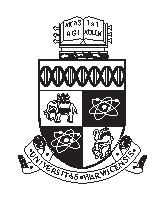
\includegraphics[width=0.4\textwidth]{crest_black.eps}
	\end{figure}
	\vspace{37mm}
	Cem Yilmaz \\
	\today
	\end{center}
	\end{titlepage}
	\tableofcontents
	\newpage
	\section{Operating Systems}
	
	\subsection{Kernel}
	\begin{tcolorbox}[colback=black!3!white,colframe=black!60!white,title=\begin{defn}Kernel \label{Kernel}\end{defn}]
	Kernel is the core of an operating system and it is loaded into the memory at system start up. It is the process running at all times on the computer. There are certain functions only a kernel performs, such as memory management, process scheduling and file handling.
	\end{tcolorbox}
	Kernel space is the part of the memory where the kernel executes. User space is the section of memory where processes run. Kernel space is kept protected from the user space and lastly, the kernel space can be accessed via user processes through system calls. These perform services like I/O operations or process creation.
	\begin{tcolorbox}[colback=black!3!white,colframe=black!60!white,title=\begin{defn}Monolithic Kernel \label{Monolithic Kernel}\end{defn}]
	The monolithic kernel contains all of the functionalities, meaning that it is a single layer kernel. Monolithic kernels make it difficult to debug the kernel code but are fast because there is little overhead in the system call interface.
	\begin{figure}[H]
		\centering
		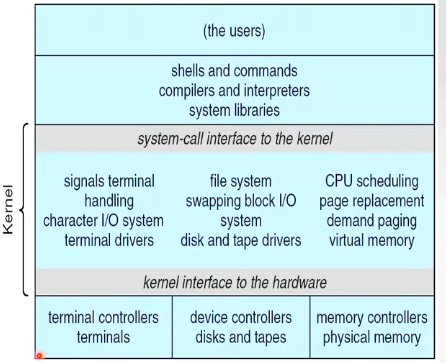
\includegraphics[width=0.7\textwidth]{one.png}
		\caption{Monolithic Kernel}
		\label{fig:one-png}
	\end{figure}
	\end{tcolorbox}
	Early OS suffered because of hardware of their time. Early hardware did not support dual mode of operation. In MS-DOS the interfaces and levels of functionality were not well defined. To combat this people have introduced layers.
	\begin{tcolorbox}[colback=black!3!white,colframe=black!60!white,title=\begin{defn}Layers \label{Layers}\end{defn}]
	Dependencies between different parts of the kernel code can be reduced using a modular kernel design approach. Modular design can be achieved through separation of different layers. The bottom layer is the hardware and the top layer is the user. Layer $K$ uses the services of layer $K-1$ and provides service to layer $K+1$ to distinguish. 
	\begin{figure}[H]
		\centering
		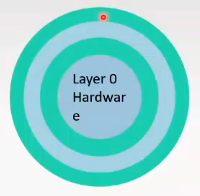
\includegraphics[width=0.3\textwidth]{two.png}
		\caption{Layer $N$ - User Interface}
		\label{fig:two-png}
	\end{figure}
	This allows developers to edit specific functionalities in specific layers only, as they're all independent.
	\begin{table}[H]
		\centering
		\caption{Layered Approach Pros and Cons}
		\label{tab:laytab}
		\begin{tabular}{|c|c|}
		\hline Pros & Cons \\
		\hline
		Simplicity of construction & Defining layers is difficult \\
		Ease of debugging & Reduced efficiency due to number of calls to execute layers \\
		Clear interface between layers & \\
		\hline
		\end{tabular}
	\end{table}
	\end{tcolorbox}
\begin{tcolorbox}[colback=black!3!white,colframe=black!60!white,title=\begin{defn}Microkernel \label{Microkernel}\end{defn}]
The Mach operating system in mid 80s modularised the kernel using a microkernel approach. The idea is to remove all non-essential components from the kernel and implement them as either system and user-level programs. These resulted in a smaller kernel. Microkernels only provided minimal process and memory management inter-process communication.
\begin{figure}[H]
	\centering
	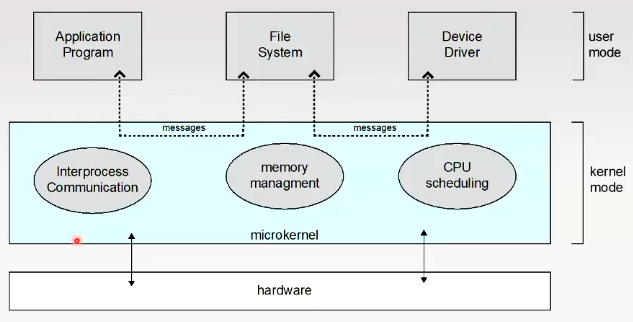
\includegraphics[width=0.8\textwidth]{three.png}
	\caption{Microkernel}
	\label{fig:three-png}
\end{figure}
	\begin{table}[H]
		\centering
		\caption{Microkernel Pros and Cons}
		\label{tab:laytab}
		\begin{tabular}{|c|c|}
		\hline Pros & Cons \\
		\hline
		Extending the operating system is easy & Efficiency - increased system call overhead \\
		Security and reliability (most processes in userspace) & \\
		\hline
		\end{tabular}
	\end{table}
\end{tcolorbox}
\begin{tcolorbox}[colback=black!3!white,colframe=black!60!white,title=\begin{defn}Loadable Kernel Module \label{Loadable Kernel Module}\end{defn}]
The most modern approach to operating system design involves loadable kernel modules. Kernel provides core services while other services are implemented dynamically as the kernel is running.
\begin{figure}[H]
	\centering
	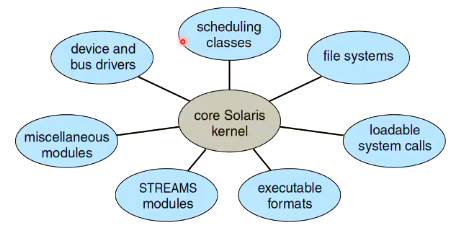
\includegraphics[width=0.7\textwidth]{four.png}
	\caption{Loadable Kernel Modules}
	\label{fig:four-png}
\end{figure}
\end{tcolorbox}
\subsection{Processes}
\begin{tcolorbox}[colback=black!3!white,colframe=black!60!white,title=\begin{defn}Process \label{Process}\end{defn}]
A process is a program in execution. A program is passive entity stored on disk as an executable file. A process is active.
\end{tcolorbox}
\begin{tcolorbox}[colback=black!3!white,colframe=black!60!white,title=\begin{exmp}Process in memory \label{Process in memory}\end{exmp}]
We present processes in memory as a continuous box of space that can be taken by text (stores instructions), data (stores global variables), heap (dynamically allocated memory), stack (stores local variables and function parameters such as return address of a function). The space between stack and heap allow them to grow or shrink during a program run-time
        \begin{figure}[H]
        	\centering
        	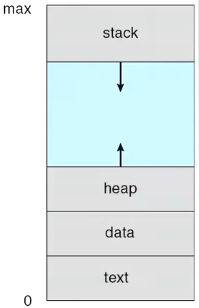
\includegraphics[width=0.2\textwidth]{five.png}
        	\caption{Virtual address space of a process}
        	\label{fig:five-png}
        \end{figure}
\end{tcolorbox}
\begin{tcolorbox}[colback=black!3!white,colframe=black!60!white,title=\begin{defn}Process Control Block (PCB) \label{Process Control Block (PCB)}\end{defn}]
The process state controls whether it is running, waiting or ready. The program counter locates the next instruction. The CPU registers contain the contents of the CPU registers i.e., CPU scheduling information (priorities, scheduling, queue pointers). Memory management information is the memory allocated to the process. Accounting information is the CPU used and time since start. I/O status is the list of open files I/O devices
\begin{figure}[H]
	\centering
	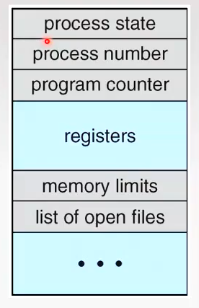
\includegraphics[width=0.2\textwidth]{six.png}
	\caption{PCB of a process}
	\label{fig:six-png}
\end{figure}
The CPU can use the PCB to switch between processes as follows
\begin{figure}[H]
	\centering
	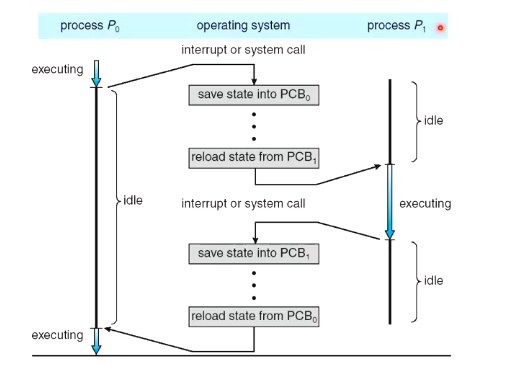
\includegraphics[width=0.8\textwidth]{seven.png}
	\caption{CPU switching between processes}
	\label{fig:seven-png}
\end{figure}
During a switch, it is a overhead and we attempt to minimise the amount of switches as much as possible.
\end{tcolorbox}
\begin{tcolorbox}[colback=black!3!white,colframe=black!60!white,title=\begin{defn}Process Scheduling \label{Process Scheduling}\end{defn}]
To maximise CPU utilisation, most modern OS support multi-programming, i.e., the ability to run multiple programs concurrently. Process scheduler selects among available processes for next execution on CPU. Some examples include:
\begin{itemize}
	\item Job queue - set of all processes in the new state
	\item Ready queue - set of all processes in the ready state
	\item Device queue - set of processes waiting for an I/O device
\end{itemize}
\end{tcolorbox}
\begin{tcolorbox}[colback=black!3!white,colframe=black!60!white,title=\begin{defn}Short-term Scheduler \label{Short-term Scheduler}\end{defn}]
The short-term schedule is invoked frequently, at least once in every 100ms. The short term scheduler must be fast. If it takes 10ms to decided to process a burst for 100 ms, then $9\%$ $(\frac{10}{110})$ of the CPU is wasted
\end{tcolorbox}
\begin{tcolorbox}[colback=black!3!white,colframe=black!60!white,title=\begin{defn}Long-Term Scheduler \label{Long-Term Scheduler}\end{defn}]
The long-term schedule is much less frequent - may be minutes between creating one process and next. The long-term scheduler controls the degree of multiprogramming (number of processes in memory). Processes can be described as either I/O bound (spends more time doing I/O then computation) or CPU bound (Long CPU bursts). A good long-term scheduler would have a good process mix. Time-sharing systems like Linux and Windows don't have a long-term schedule. Everything is dumped to the short-term scheduler.
\end{tcolorbox}
\begin{tcolorbox}[colback=black!3!white,colframe=black!60!white,title=\begin{defn}Process Creation \label{Process Creation}\end{defn}]
An OS must provide ways for users to create new processes. A system process (parent) creates a user process (child). The OS provides system calls for a user process to create another process. For example, in UNIX-based operating systems, processes can be created using the $fork\left(  \right) $ system call.
\end{tcolorbox}
\begin{tcolorbox}[colback=black!3!white,colframe=black!60!white,title=\begin{exmp}Fork() \label{Fork()}\end{exmp}]
\begin{figure}[H]
	\centering
	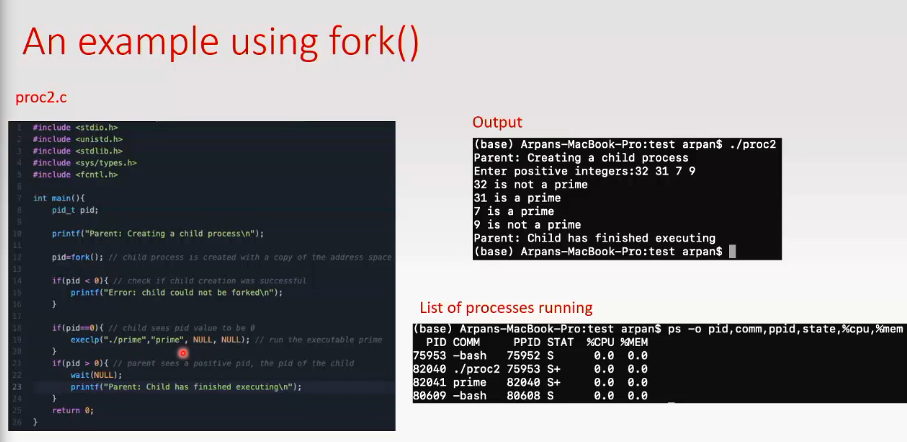
\includegraphics[width=1\textwidth]{eight.png}
	\caption{Fork example}
	\label{fig:eight-png}
\end{figure}
\begin{figure}[H]
	\centering
	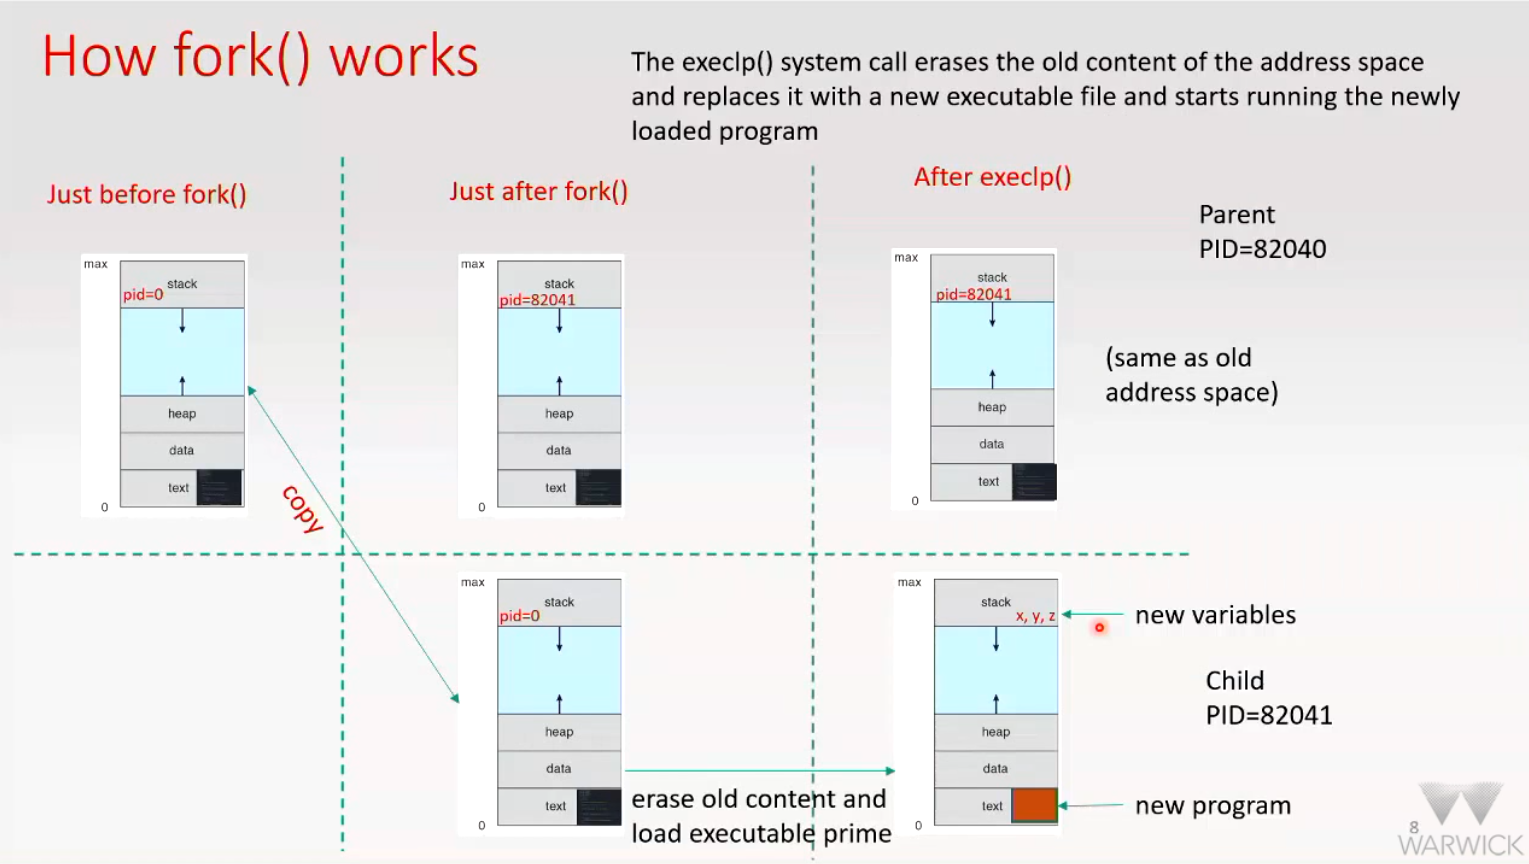
\includegraphics[width=1\textwidth]{nine.png}
	\caption{Fork system and execlp}
	\label{fig:ninenine-pngpng}
\end{figure}
\end{tcolorbox}
\begin{tcolorbox}[colback=black!3!white,colframe=black!60!white,title=\begin{defn}Process Termination \label{Process Termination}\end{defn}]
A parent process may terminate the execution of child processes using the $abort\left(  \right) $ system call. Some examples include that child has exceeded its allocated resources. Task assigned to child is no longer required. The parent is exiting and the operating system does not allow a child to continue if its parent terminates.
\end{tcolorbox}
\subsection{Interprocess Communication (IPC)}
\begin{tcolorbox}[colback=black!3!white,colframe=black!60!white,title=\begin{defn}Interprocess Communication (IPC) \label{Interprocess Communication (IPC)}\end{defn}]
Processes running concurrently may want to communicate with each other. For example, when two processes are working on a task together, they may need to share data. The data produced by one process may be required by other processes. There are two ways to achieve this:
\begin{itemize}
	\item Shared memory - a region of memory that is shared by communicating processes is established
	\item Message passing - messages are exchanged between the communicating processes
\end{itemize}
\begin{figure}[H]
	\centering
	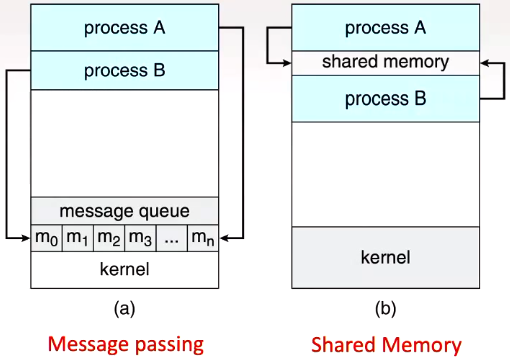
\includegraphics[width=0.8\textwidth]{ten.png}
	\caption{Message Passing vs Shared Memory}
	\label{fig:ten-png}
\end{figure}
For message passing, processes interact by sending messages to each other. The kernel provides a logical communication channel and systems calls are used to pass messages. 

For shared memory, processes interact by writing to or reading from a shared part of the memory. The kernel is involved only in establishing the shared part of memory; communication is entirely handled by the communication processes.
\end{tcolorbox}
\begin{tcolorbox}[colback=black!3!white,colframe=black!60!white,title=\begin{defn}Shared Memory \label{Shared Memory}\end{defn}]
Shared memory resides in the address space of one of the communicating processes. Other process need permission to access it. Kernel is required to setup shared memory and grant permission. Once shared memory is established, processes are responsible for maintaining proper synchronisation.
\begin{figure}[H]
	\centering
	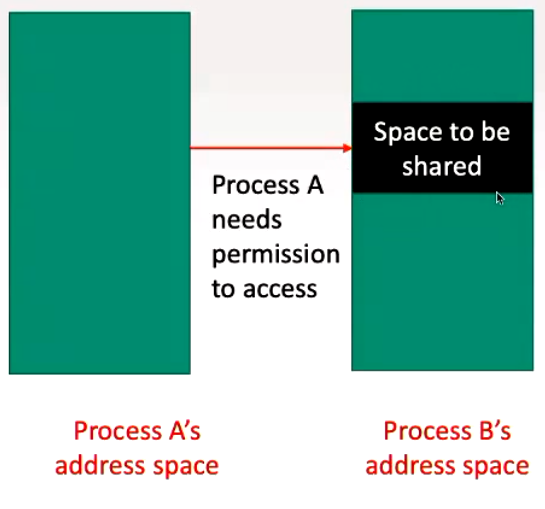
\includegraphics[width=0.4\textwidth]{eleven.png}
	\caption{Shared Memory}
	\label{fig:eleven-png}
\end{figure}
\end{tcolorbox}
\begin{tcolorbox}[colback=black!3!white,colframe=black!60!white,title=\begin{defn}Producer-Consumer Paradigm \label{Producer-Consumer Paradogim}\end{defn}]
The shared buffer/memory space can be filled by the producer and emptied by a consumer. Consumer must wait when the buffer is empty. Producer must wait when the buffer is full. When the buffer space is practically unbounded, this is not an issue.
\end{tcolorbox}
\begin{tcolorbox}[colback=black!3!white,colframe=black!60!white,title=\begin{defn}Message Passing Systems \label{Message Passing Systems}\end{defn}]
A message passing system should at least provide two operations:
\begin{itemize}
	\item send(message)
	\item receive(message)
\end{itemize}
These are generally implemented using system calls. Processes must name each other explicitly:
send (P, message)
and receive(Q, message) or receive(id,message). We have a message in the receive so we can store the message. Links are established automatically and a link is associated with exactly one pair of communicating processes. Hard coding the processes identifier may not be ideal since every time a process is run its id can change. Or, it can be created using a mailbox system where
send(mailboxid, message) and receive(mailboxid, message) is implemented. A shared mailbox is found in kernel with a specific ID named mailboxid. This is called indirect communication as we specify the mailbox instead of the process IDs. We can synchronise these messages by using blocking.
\begin{itemize}
	\item Blocking send - the sender is blocked until the message is received
	\item Blocking receive - the receiver is blocked until a message is available
\end{itemize}
\end{tcolorbox}
\begin{tcolorbox}[colback=black!3!white,colframe=black!60!white,title=\begin{defn}Buffering \label{Buffering}\end{defn}]
Communication link is a buffer. Implementation of send() and receive() depends on the capacity of this buffer
\begin{itemize}
	\item Zero capacity - the queues a maximum length of zero, so sender must block until recipient receives the message
	\item Bounded capacity - the queue has a finite length, when full the sender must be blocked
	\item Unbounded capacity - the queue's length is potentially infinite. Sender never blocks.
\end{itemize}
\end{tcolorbox}
\begin{tcolorbox}[colback=black!3!white,colframe=black!60!white,title=\begin{exmp}Examples of IPC \label{Examples of IPC}\end{exmp}, breakable, enhanced]
\begin{defn}
	mmap
\end{defn}
\begin{figure}[H]
	\centering
	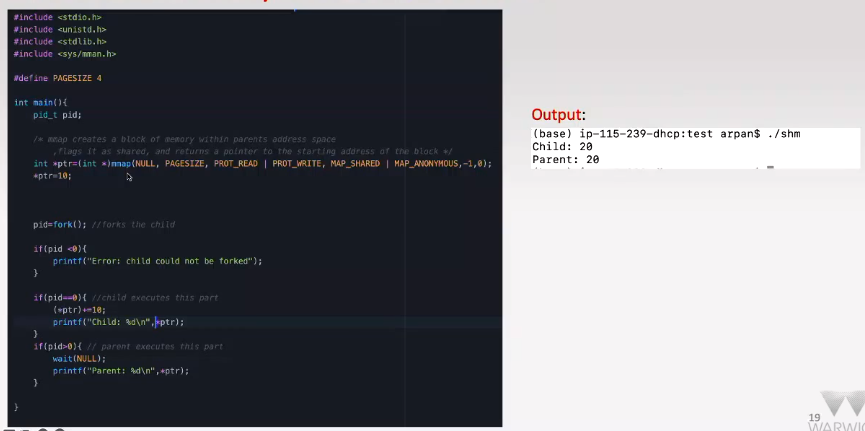
\includegraphics[width=1\textwidth]{twelve.png}
	\caption{Shared Memory Communication using mmap}
	\label{fig:twelve-png}
\end{figure}        
The mmap allocates memory in the memory address. Note that malloc uses mmap in its implementation.
\begin{defn}
	Ordinary Pipes
\end{defn}
Ordinary pipes in UNIX allow simple one-way communication through message passing. A pipe connects the output of one process to the input of another process. In UNIX systems, pipes are commonly created within bash terminal using |. 
\begin{figure}[H]
	\centering
	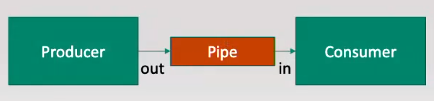
\includegraphics[width=0.5\textwidth]{thirteen.png}
	\caption{Ordinary pipe}
	\label{fig:thirteen-png}
\end{figure}
\begin{figure}[H]
	\centering
	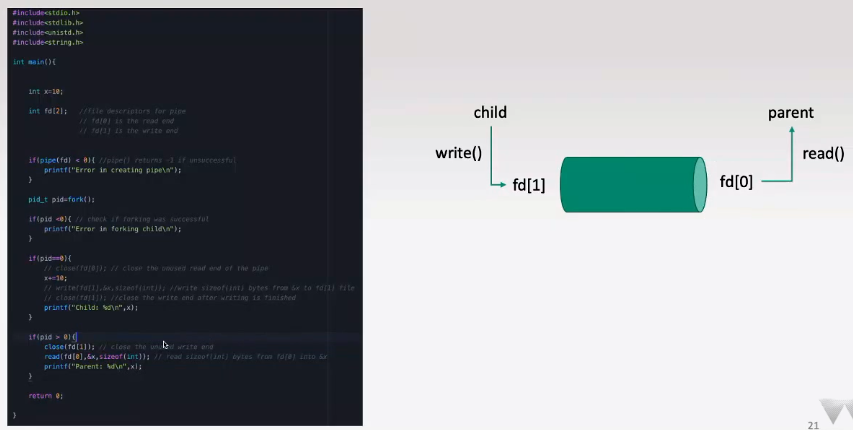
\includegraphics[width=1\textwidth]{fourteen.png}
	\caption{Ordinary Pipe in C}
	\label{fig:fourteen-png}
\end{figure}
In the figure above, fd is a pipe that is used by the child created using fork. There is an error in the code where write should be uncommented. The write line inserts the new value of $x$ into fd[1].
\begin{defn}
	Named Pipes
\end{defn}
\begin{figure}[H]
	\centering
	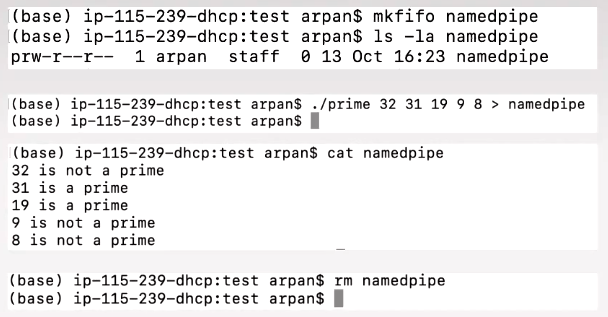
\includegraphics[width=1\textwidth]{fifteen.png}
	\caption{Named Pipes in UNIX}
	\label{fig:fifteen-png}
\end{figure}
Named pipes are similar to files that store information, except they're not files and are separate allowing them to be faster.
\end{tcolorbox}
\subsection{Threading}
\begin{tcolorbox}[colback=black!3!white,colframe=black!60!white,title=\begin{defn}Thread \label{Thread}\end{defn}]
A thread is a unit of CPU execution. Single-threaded process: one chain of execution running each line sequentially. If we have multiple similar tasks, one solution is to run the same function in a loop for each task. To achieve concurrency, create a separate process for each task, but it's not efficient. Each process requires its own address space in memory. Code, data could be shared. The benefits of threads include
\begin{itemize}
	\item Economy - cheaper than process creation, thread switching lower overhead than context switching
	\item Scalability - large number of concurrent tasks
	\item Responsiveness - may allow continued execution of one thread even when another thread is blocked
	\item Resource sharing - threads share resources of process, easier than shared memory or message passing i.e., easy communication between threads
\end{itemize}
\end{tcolorbox}
\begin{tcolorbox}[colback=black!3!white,colframe=black!60!white,title=\begin{defn}Multithreading \label{Multithreading}\end{defn}]
Multithreaded programs are when each thread perform a separate task from a single process. They share the same code, data and files as they're from a single process. Threads share more things with their parents than processes do i.e., code, data, heap, opened files, signals etc. Each thread is comprised of a thread id, program counter, a register set and a stack. A thread creation has less overhead as it shares a lot of things.
\end{tcolorbox}
\begin{tcolorbox}[colback=black!3!white,colframe=black!60!white,title=\begin{defn}Concurrency vs Parallelism \label{Concurrency vs Parallelism}\end{defn}]
Concurrency supports more than one task making progress. A single CPU system may appear to be running tasks concurrently by interleaving their execution. \\
Parallelism implies that a system can perform more than one task simultaneously. 
\begin{figure}[H]
	\centering
	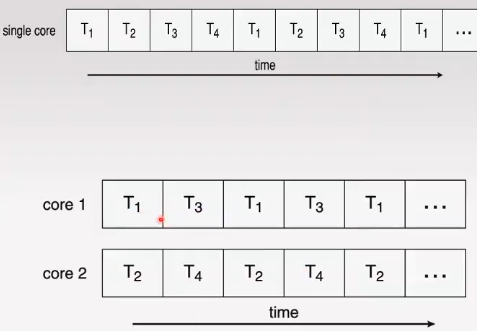
\includegraphics[width=0.6\textwidth]{twentyseven.png}
	\caption{Concurrency vs parallelism}
	\label{fig:twentyseven-png}
\end{figure}
\end{tcolorbox}
\begin{tcolorbox}[colback=black!3!white,colframe=black!60!white,title=\begin{defn}Data parallelism and task parallelism \label{Data parallelism and task parallelism}\end{defn}]
Data parallelism distributes subsets of the same data across multiple cores, performing the same operation each core. \\
In task parallelism, it splits threads performing different tasks across multiple cores. \\
Applications can have a mix of both types.
\begin{figure}[H]
	\centering
	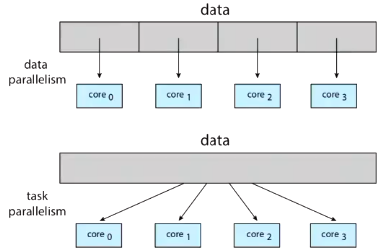
\includegraphics[width=0.8\textwidth]{twentyeight.png}
	\caption{Data vs task parallelism}
	\label{fig:twentyeight-png}
\end{figure}
\end{tcolorbox}
\begin{tcolorbox}[colback=black!3!white,colframe=black!60!white,title=\begin{thm}Amdahl's Law \label{Amdahl's Law}\end{thm}]
	Amdahl's law helps us compute the speed up obtained by parallelism
		\begin{align}	
		\text{speedup}\le \frac{1}{S+\frac{1-S}{N}}
		\end{align}
Where time taken to run the serial part is $0\le S\le 1$ and the $1$ in numerator expresses the time taken before parallelising. The $\frac{1-S}{N}$ is the time taken to run the parallelisable part with $N$ cores
\end{tcolorbox}
\begin{tcolorbox}[colback=black!3!white,colframe=black!60!white,title=\begin{defn}Thread Synchronosation \label{Thread Synchronosation}\end{defn}]
When multiple threads write to the same location, we must synchronise the threads. Synchronisation ensure that one thread does not overwrite the contents written by the other thread.
\end{tcolorbox}
\begin{tcolorbox}[colback=black!3!white,colframe=black!60!white,title=\begin{exmp}Thread Sync \label{Thread Sync}\end{exmp}]
        Assume two threads, Thread $1$ and Thread $2 $. They both try to update a global variable, $sum$. Thread $1$ does
	\begin{align*}
		sum=sum+i
	\end{align*}
	Thread 2 does
	\begin{align*}
		sum=sum+j
	\end{align*}
Assume they do this in a concurrent manner. Atomically, we have
\begin{align*}
	register 1 = sum \;\;\;\;\;&\;\;\;\;\; register 2 = sum \\
	register 1 = register 1 + i \;\;\;\;\; & \;\;\;\;\;register 2 = register 1 + j \\
	sum = register 1 \;\;\;\;\;&\;\;\;\;\; sum = register 2 
\end{align*}
which results in wrong result, that is, for example, where $sum=0$, $i=1$ and $j=5001$
\begin{figure}[H]
	\centering
	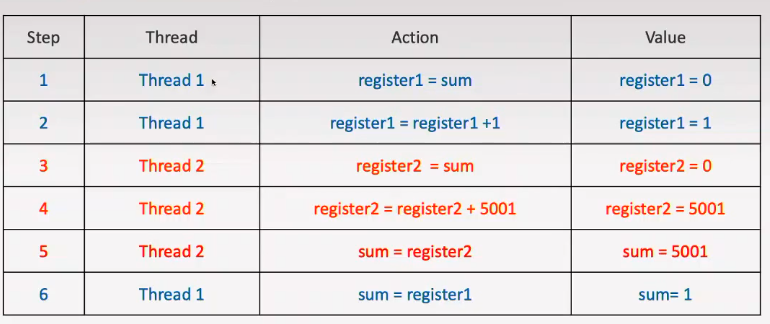
\includegraphics[width=0.8\textwidth]{twentynine.png}
	\caption{Order of operations without sync}
	\label{fig:twentynine-png}
\end{figure}
From the table above, we can see that the value from Thread $2$ is lost. This is error is called Race condition. Threads engage in a race to become the last one to write on the shared variable sum. Only one of the values is preserved. Race conditions should be avoided by proper synchronisation.
\end{tcolorbox}
\begin{tcolorbox}[colback=black!3!white,colframe=black!60!white,title=\begin{defn}Mutex Locks \label{Mutex Locks}\end{defn}]
There are many ways to synchronise threads. One common way is use mutual exclusion locks or mutex locks. The idea is that each thread must first acquire a lock to perform updates on shared variables, called the critical section. 
\begin{figure}[H]
	\centering
	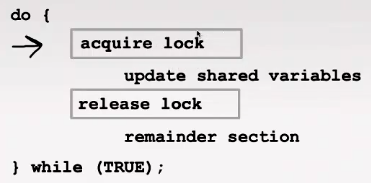
\includegraphics[width=0.4\textwidth]{thirty.png}
	\caption{Mutex Lock}
	\label{fig:thirty-png}
\end{figure}
\end{tcolorbox}
\begin{tcolorbox}[colback=black!3!white,colframe=black!60!white,title=\begin{defn}User-level and Kernel level threads \label{User-level and Kernel level threads}\end{defn}]
Kernel itself may be multi-threaded and some kernel threads provide services to users and others are used to run user processes. Kernel can schedule them on different CPUs. \\

For user-level threads, they exist within a user process if they are multi-threaded. For a user-level thread to execute on a CPU, it must be associated with a kernel-level thread.
\begin{figure}[H]
	\centering
	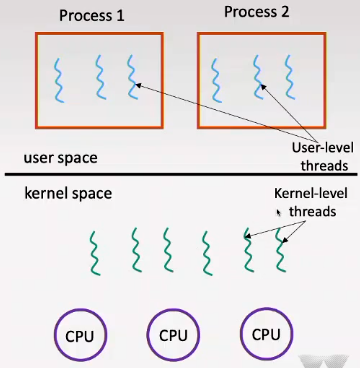
\includegraphics[width=0.8\textwidth]{thirtyone.png}
	\caption{User-level and Kernel-level threads}
	\label{fig:thirtyone-png}
\end{figure}
\end{tcolorbox}

\begin{tcolorbox}[colback=black!3!white,colframe=black!60!white,title=\begin{defn}One-to-one model \label{One-to-one model}\end{defn}]
Each user-level thread maps to a kernel thread. Linux and windows use this. The advantages include
\begin{itemize}
	\item Kernel is aware of all the threads running within the user process. Hence, we can rely on the kernel to schedule these threads on different CPUs.
\end{itemize}
The disadvantage includes
\begin{itemize}
	\item Creating each user-level thread involves the kernel, meaning it is expensive.
	\item User is limited by the support provided by the kernel to manage threads.
\end{itemize}
\end{tcolorbox}
\begin{tcolorbox}[colback=black!3!white,colframe=black!60!white,title=\begin{defn}Many-to-one model \label{Many-to-one model}\end{defn}]
The many to one model is when many user level threads are mapped to a single kernel thread.
Advantages are:
\begin{itemize}
	\item Less overhead and more flexibility in thread management
\end{itemize}
The disadvantages include:
\begin{itemize}
	\item Multiple threads may not run in parallel, because only one may be in kernel at a time
	\item One blocking thread causes all to block
\end{itemize}
\end{tcolorbox}
\begin{tcolorbox}[colback=black!3!white,colframe=black!60!white,title=\begin{defn}Many-tomany model \label{Many-tomany model}\end{defn}]
Mixture of one-to-one and many-to-one models. Allow user-level threads to be multiplexed onto smaller or equal number of kernels level threads. The advantages include
\begin{itemize}
	\item Kernel threads can run in parallel, blocking call by one user-level thread does not block the entire process
	\item Programmers can decide how many kernel threads to use and how many user level threads should be mapped to each one, causing less overhead.
\end{itemize}
\end{tcolorbox}
\begin{tcolorbox}[colback=black!3!white,colframe=black!60!white,title=\begin{defn}One thread-per-request strategy \label{One thread-per-request strategy}\end{defn}]
Server creating a separate thread to handle each client request. This causes
\begin{itemize}
	\item High overhead for each thread
	\item High traffic will create a large number of threads, slowing down the system by burdening it.
\end{itemize}
\begin{figure}[H]
	\centering
	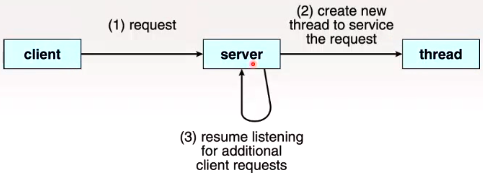
\includegraphics[width=0.8\textwidth]{thirtytwo.png}
	\caption{1 TPS strategy}
	\label{fig:thirtytwo-png}
\end{figure}
\end{tcolorbox}
\begin{tcolorbox}[colback=black!3!white,colframe=black!60!white,title=\begin{defn}Thread Pool Strategy \label{Thread Pool Strategy}\end{defn}]
The thread pool strategy involves the main server thread, which creates a predefined number $n$ of worker threads. The number $n$ usually does not change. Instead, we map existing $n$ threads to serve new requests. When pool of thread workers are full, the main server thread creates a queue of pending requests. 
\begin{figure}[H]
	\centering
	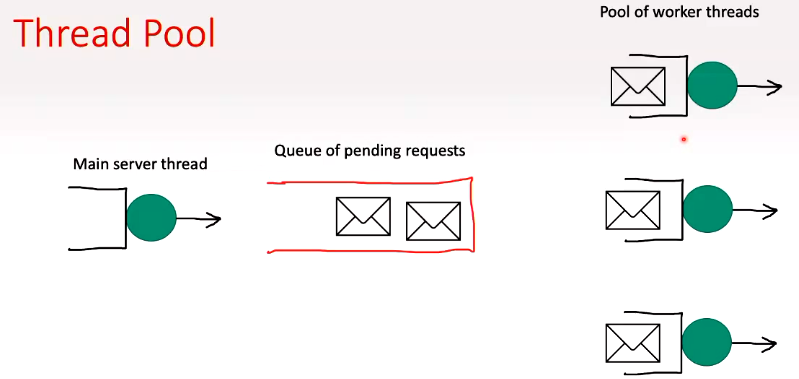
\includegraphics[width=0.8\textwidth]{thirtythree.png}
	\caption{Thread Pool}
	\label{fig:thirtythree-png}
\end{figure}
The advantages include
\begin{itemize}
	\item Usually slightly faster to service a request with an existing thread than create a new thread
	\item Allows the number of threads in the application to be bound to the size of the pool. This size is decided by the programmer taking into account the number of processing cores, memory in use, expected number of client requests etc.
\end{itemize}
Disadvantages are
\begin{itemize}
	\item A request may have to wait in a queue if all workers are busy
	\item Deciding the number of workers in a threadpool is not easy. May have to be adjusted dynamically depending on load.
\end{itemize}
\end{tcolorbox}
\begin{tcolorbox}[colback=black!3!white,colframe=black!60!white,title=\begin{defn}Signal Handling \label{Signal Handling}\end{defn}]
Signals are used in UNIX systems to notify a process about the occurrence of certain events. Type of signals include synchronous i.e., internally generated by a process such as division by $0$. And asynchronous which is externally generated such as terminating a process with CTRL+C sends signal SIGINT. All signals follow the same pattern: it is generated, delivered to the process, and handled by the process. Signal is handled by one of two signal handlers:
\begin{itemize}
	\item Default - every signal has default handler that kernel runes when handling signal e.g. SIGINT
	\item User-defined - user defined signal handler can override default
\end{itemize}
In multi-threaded programs, a signal be delivered to all threads or specific threads. Synchronous signals are generally delivered to thread generating the signal. Some asynchronous signals like SIGINT should be sent to all threads. Signal can also be delivered to a specific process.
\end{tcolorbox}
\subsection{Scheduling}
\begin{tcolorbox}[colback=black!3!white,colframe=black!60!white,title=\begin{defn}CPU and I/O bursts \label{CPU and I/O bursts}\end{defn}]
Goal of CPU scheduling is to increase CPU utilisation. Life of a process is CPU burst followed by I/O burst. When a process is in a I/O burst, the CPU can be scheduled to some other process.
\end{tcolorbox}
\begin{tcolorbox}[colback=black!3!white,colframe=black!60!white,title=\begin{defn}Performance Measures \label{Performance Measures}\end{defn}]
The performance measures for CPU include:
\begin{itemize}
	\item CPU Utilisation - fraction/percentage of time CPU remains busy when there are jobs in the ready queue
	\item Throughput - number of processes that complete their execution per time unit
	\item Turnaround time - amount of time to complete a process
	\item Waiting time - amount of time a process spends waiting in the ready queue
	\item Response time - amount of time it takes from when a request was submitted until the first response is produced
\end{itemize}
\end{tcolorbox}
\begin{tcolorbox}[colback=black!3!white,colframe=black!60!white,title=\begin{defn}Types of scheduling \label{Types of scheduling}\end{defn}]
There are two types of scheduling:
\begin{itemize}
	\item Non-preemptive - once the cpu is given to a process, the process holds onto the CPU until its current CPU burst finishes.
	\item Preemptive - the execution of a process is interrupted in the middle to schedule another process
\end{itemize}
Most modern OS use preemptive algorithms. Preemptive algorithms, however, have their own issues. Pre-emptive scheduling can cause race conditions. If a process is pre-empted while it is updating some shared data then it leaves data in an inconsistent state. Another process is scheduled which accesses the same data then it will leave it in an inconsistent state again. Shared data should be updated within critical sections using proper synchronisation primitives.
\end{tcolorbox}
We will now discuss scheduling algorithms
\begin{tcolorbox}[colback=black!3!white,colframe=black!60!white,title=\begin{defn}First Come First Serve (FCFS) \label{First Come First Serve (FCFS)}\end{defn}]
Processes are assigned to the CPU in order of their arrivals.
\begin{figure}[H]
	\centering
	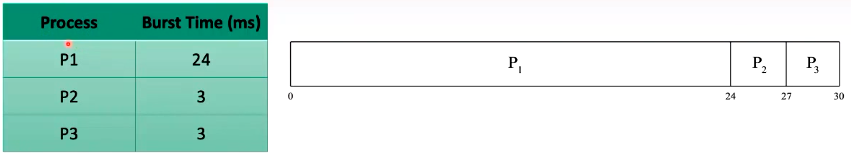
\includegraphics[width=0.8\textwidth]{thirtysix.png}
	\caption{FCFS Scheduler}
	\label{fig:thirtysix-png}
\end{figure}
The waiting time for the above information is $0$ ms for P1, $24$ ms for P2 and $27$ ms for P3, meaning that the average waiting time is
 \begin{align*}
	 \frac{0+24+27}{3}=17\text{ms}	
\end{align*}
\end{tcolorbox}
\begin{tcolorbox}[colback=black!3!white,colframe=black!60!white,title=\begin{defn}Shorest Job First (SJF) \label{Shorest Job First (SJF)}\end{defn}]
The process with the shortest next CPU burst is selected. (If there is a tie, we use FCFS).
\begin{figure}[H]
	\centering
	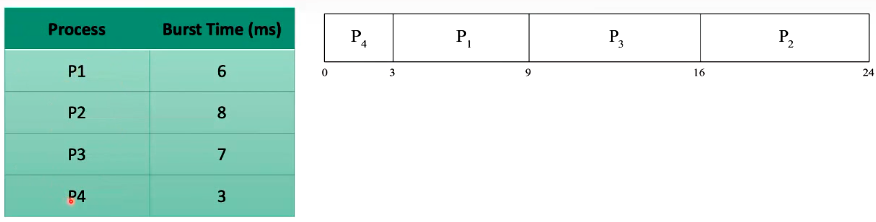
\includegraphics[width=0.8\textwidth]{thirtyseven.png}
	\caption{SJF}
	\label{fig:thirtyseven-png}
\end{figure}
The average waiting time is
\begin{align*}
	\frac{0+3+9+16}{4}=7\text{ms}
\end{align*}
In comparison, FCFS would've computed us an average of $10.25$ ms. 
SJF is provably optimal, in that it gives the minimum average time. The problem is knowing how long the next CPU burst will be can only be an estimate. There are also two versions of SJF, which are pre-emptive and non-pre-emptive. Pre-emptive SJF switches to newly arrived process and non-pre-emptive SJF will allow the current existing job to finish.
\begin{figure}[H]
	\centering
	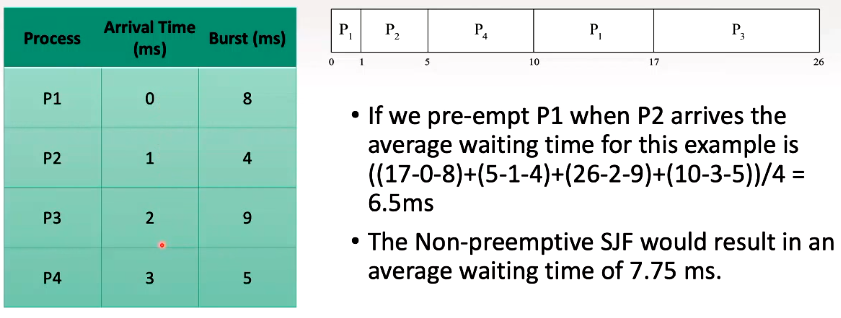
\includegraphics[width=0.8\textwidth]{thirtyeight.png}
	\caption{Preemptive SJF}
	\label{fig:thirtyeight-png}
\end{figure}
\end{tcolorbox}
\begin{tcolorbox}[colback=black!3!white,colframe=black!60!white,title=\begin{defn}Priority Scheduling \label{Priority Scheduling}\end{defn}]
SJF is a special case of priority scheduling. A priority is associated with each process and CPU is allocated to the highest priority process. Priorities can be indicated by numbers. In SJF, priorities are the next CPU burst times. \\

However, priority schedule comes with a problem called starvation. Very low priority processes may never get scheduled. A fix to this is aging, gradually increasing the priority of processes that wait in the system for a long time.
\end{tcolorbox}
\begin{tcolorbox}[colback=black!3!white,colframe=black!60!white,title=\begin{defn}Round Roubin (RR) Scheduling \label{Round Roubin (RR}\end{defn}]
Each process gets a small unit of CPU time called time quantum $q$. After this time has elapsed, the process is preempted and added to the end of the ready queue. Generally, the schedule visits the processes in order of their arrivals. If there are $N$ processes in the ready queue and the time quantum is $q$, then each process gets $\frac{1}{N}$ of the CPU time in chunks of at most $q$ time units at once. No process waits more than $\left( N-1 \right) q$ time units for its next turn. Note that RR is naturally preemptive. If $q$ is large, then it imitates the behaviour of FCFS. If  $q$ is small, then there are too many context switches. $q$ is usually $10$ ms to $100$ ms.
\begin{figure}[H]
	\centering
	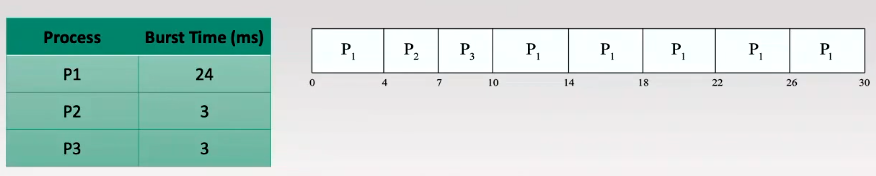
\includegraphics[width=0.8\textwidth]{thirtynine.png}
	\caption{RR schedule with $q=4$}
	\label{fig:thirtynine-png}
\end{figure}
In the above figure example, we have that the average waiting time is
\begin{align*}
	\frac{\left( 30-0-24 \right) +\left( 7-0-3 \right) +\left( 10-0-3 \right) }{3} = 5.66\text{ms}
\end{align*}
The waiting time using FCFS is $17$ ms but SJF is $3$ ms. Despite there is higher average waiting time than SJF, there is better response.
\end{tcolorbox}
\begin{tcolorbox}[colback=black!3!white,colframe=black!60!white,title=\begin{thm}Exponential Moving Average \label{Exponential Moving Average}\end{thm}]
	\begin{enumerate}
		\item $t_n = $ actual length of $n^{th}$ CPU burst
		\item $\tau_{n+1}=$ predicted value of the next CPU burst
		\item $\alpha, 0\le \alpha\le 1$ 
		\item $\tau_{n+1} = \alpha t_n + (1-\alpha)\tau_n$
	\end{enumerate}
	Expanding the recursion gives
		\begin{align}
		\tau_{n+1} = \alpha t_n + (1-\alpha)\alpha t_{n-1} + \ldots + (1-\alpha)^{j}\alpha t_{n-j} + \ldots + (1-\alpha)^{n+1}\tau_0
		\end{align}
\end{tcolorbox}
\subsection{Synchronisation}
Synchronisation is required for threads as discussed before. However, processes may need it as well e.g., shared memory. In this case, we will refer to processes as both processes and threads, as the solutions and problems are the same.
\begin{tcolorbox}[colback=black!3!white,colframe=black!60!white,title=\begin{defn}Critical Section \label{Critical Section}\end{defn}]
Critical section is part of the code where shared variables are updated.
\end{tcolorbox}
When one process is in a critical section, no other process should be allowed in its critical section (mutual exclusion). 
\begin{tcolorbox}[colback=black!3!white,colframe=black!60!white,title=\begin{defn}The Critical Section Problem \label{The Critical Section Problem}\end{defn}]
Consider a group of process
\begin{align*}
	\{P_0,P_1,\ldots,P_N\}
\end{align*}
Each process has a critical section of code where they update some shared variables. The critical section problem: \\
\textbf{Design a protocol such that no two processes can concurrently execute their critical sections}. \\
Mutual exclusion is not the only criteria that we must satisfy. We must also catch its progress. If no process is executing in its critical and there exist some processes that wish to enter their critical section, then one of the waiting processes must be able to enter into its critical section. The last criteria is the bounded waiting criteria. No one process should have to wait indefinitely to enter its critical section while other processes are being allowed to enter and exit their critical sections continually. Note that the bounded waiting is a stronger requirement than progress requirement. 
\end{tcolorbox}
\begin{tcolorbox}[colback=black!3!white,colframe=black!60!white,title=\begin{exmp}Possible solution for two processes \label{Possible solution for two processes}\end{exmp}]
        Consider two processes $P_0$ and $P_1$. One basic solution is to create a shared variable called "turn", a $0$ or $1$. 
	\begin{figure}[H]
		\centering
		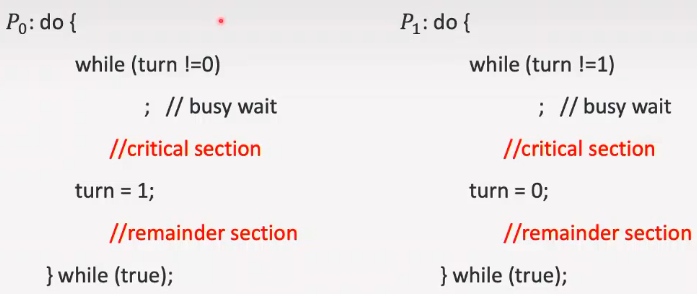
\includegraphics[width=0.7\textwidth]{fourty.png}
		\caption{Turn solution}
		\label{fig:fourty-png}
	\end{figure}
	Whilst this solution provides mutual exclusion, if $P_1$ finished whilst $P_0$ still has to edit the critical section, $P_0$ will not be able to access its critical section. Another solution is proposed by Gary L. Peterson in 1981. The solution involves the following logic:
	\begin{figure}[H]
		\centering
		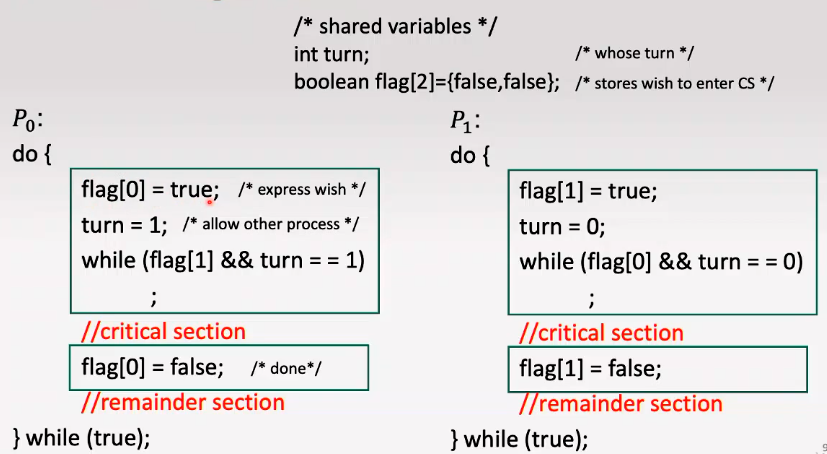
\includegraphics[width=0.8\textwidth]{fourtyone.png}
		\caption{Peterson's Algorithm}
		\label{fig:fourtyone-png}
	\end{figure}
Peterson's algo satisfies all three criteria but it is not perfect. It employs busy and may fail in modern architectures, as the order of array and turn may switch causing it to fail.
\end{tcolorbox}
\begin{tcolorbox}[colback=black!3!white,colframe=black!60!white,title=\begin{defn}Locks \label{Locks}\end{defn}]
We now explore more practical techniques to solve the CS problem. All solutions are based on idea of locking, i.e., two processes can not have a lock simultaneously. 
\begin{figure}[H]
	\centering
	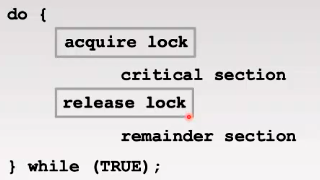
\includegraphics[width=0.4\textwidth]{fourtytwo.png}
	\caption{Locks}
	\label{fig:fourtytwo-png}
\end{figure}
Locks should be atomic, meaning non-interruptible. Modern machines provide special atomic hardware instructions to implement locks. An example is $\text{test}\_\text{and}\_\text{set}$
\end{tcolorbox}
\begin{tcolorbox}[colback=black!3!white,colframe=black!60!white,title=\begin{exmp}Test and set Instruction \label{Test and set Instruction}\end{exmp}]
        The set and set instruction, by definition, returns original value of passed parameter $target$. Set the new value of passed parameter $target$ to "TRUE". It needs to be implemented atomically using hardware.
	\begin{figure}[H]
		\centering
		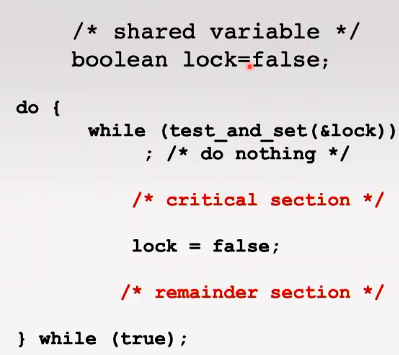
\includegraphics[width=0.4\textwidth]{fourtythree.png}
		\caption{Test and set solution}
		\label{fig:fourtythree-png}
	\end{figure}
	\begin{figure}[H]
		\centering
		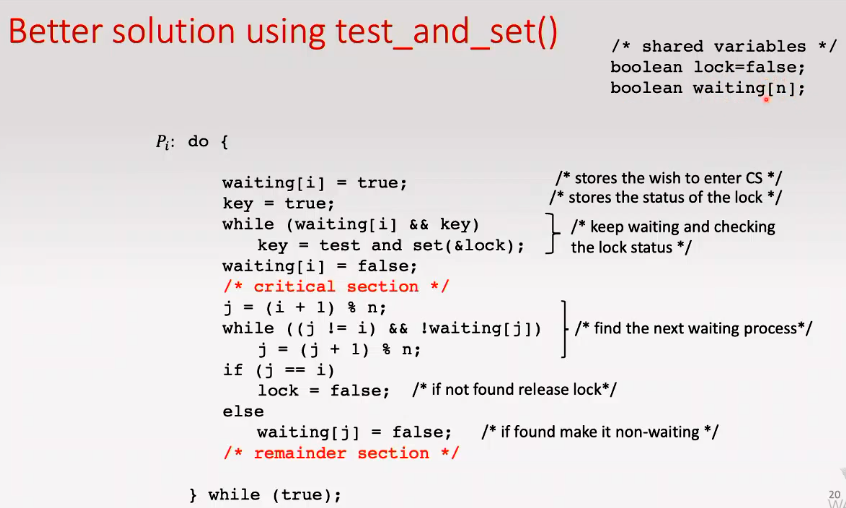
\includegraphics[width=0.8\textwidth]{fourtyfour.png}
		\caption{Better solution}
		\label{fig:fourtyfour-png}
	\end{figure}
\end{tcolorbox}
\begin{tcolorbox}[colback=black!3!white,colframe=black!60!white,title=\begin{defn}Synchronisation Primitives \label{Synchronisation Primitives}\end{defn}]
Hardware based solutions are generally inaccessible to programmers. OS designers build software tools to solve critical section problem. These are the synchronisation primitives:
\begin{itemize}
	\item Mutex Locks
	\item Condition Variables
	\item Semaphores
\end{itemize}
\end{tcolorbox}
\begin{tcolorbox}[colback=black!3!white,colframe=black!60!white,title=\begin{defn}Mutex Lock \label{Mutex Lock}\end{defn}]
\begin{figure}[H]
	\centering
	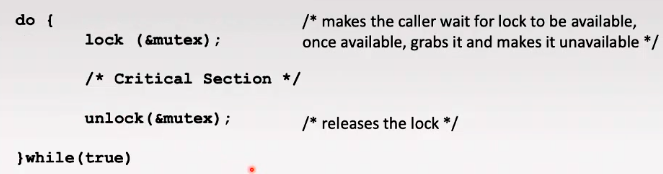
\includegraphics[width=0.8\textwidth]{fourtyfive.png}
	\caption{Mutex Lock}
	\label{fig:fourtyfive-png}
\end{figure}
The mutex lock has two operations available: the lock and unlock. The lock operation it makes other processes wait for the mutex lock to be available. Once it is available, a process is available to acquire that lock and makes mutex unavailable to other processes. It then executes the critical section and finally releases the lock. Functionally, the lock must be implemented with two fields: a boolean lock, and a list that list the processes waiting on the mutex. 
\begin{figure}[H]
	\centering
	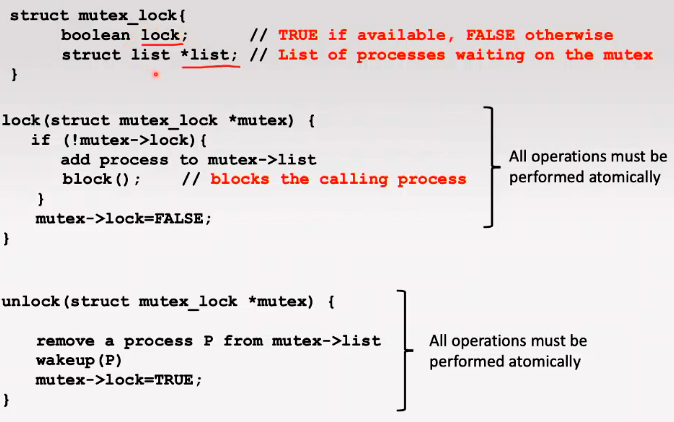
\includegraphics[width=0.8\textwidth]{fourtysix.png}
	\caption{Mutex Lock Implementation}
	\label{fig:fourtysix-png}
\end{figure}
Initially, the lock command first checks if mutex is locked. If locked, it adds the process onto the list and we block that process, meaning that the process goes to sleep. The unlock operation removes a process $P$ from the list, wakes up that process $P$, and sets the value of lock to true. 
\end{tcolorbox}
\begin{tcolorbox}[colback=black!3!white,colframe=black!60!white,title=\begin{defn}Semaphores \label{Semaphores}\end{defn}]
Semaphores can have integer values, meaning that they're more powerful than mutex locks. A zero value indicates that the semaphore is not available. Positive values indicate that it is available. It can only be accessed via two indivisible atomic operations $wait\left(  \right) $ and $signal\left(  \right) $.
The operations are as following:
\begin{itemize}
	\item $wait\left(  \right) $- checks if the value of the semaphore is $\le 0$ and if so it makes the calling process wait until it becomes positive
	\item Once the semaphore value is positive $wait\left(  \right) $ function decrements it by $1$.
	\item $signal\left(  \right) $ function increments the value of the semaphore by $1$ 
	\item Both $wait\left(  \right) $ and $signal\left(  \right) $ must be performed atomically
\end{itemize}
\begin{figure}[H]
	\centering
	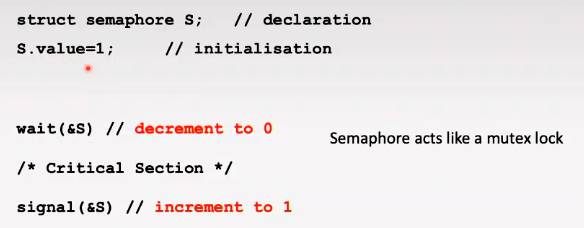
\includegraphics[width=0.6\textwidth]{fourtyseven.png}
	\caption{Semaphore as mutex}
	\label{fig:fourtyseven-png}
\end{figure}
\begin{figure}[H]
	\centering
	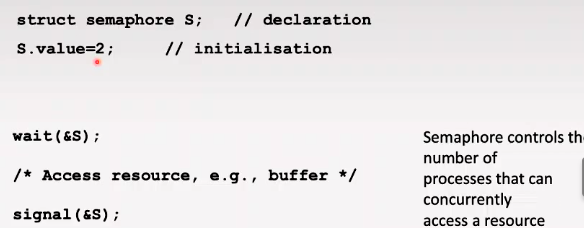
\includegraphics[width=0.6\textwidth]{fourtyeight.png}
	\caption{Semaphore with higher number}
	\label{fig:fourtyeight-png}
\end{figure}
Semaphores can also be initialised with a higher number if we want processes to access shared memory simultaneously. The implementation is similar to that of mutex, however, we change the boolean statement to an integer instead as follows
\begin{figure}[H]
	\centering
	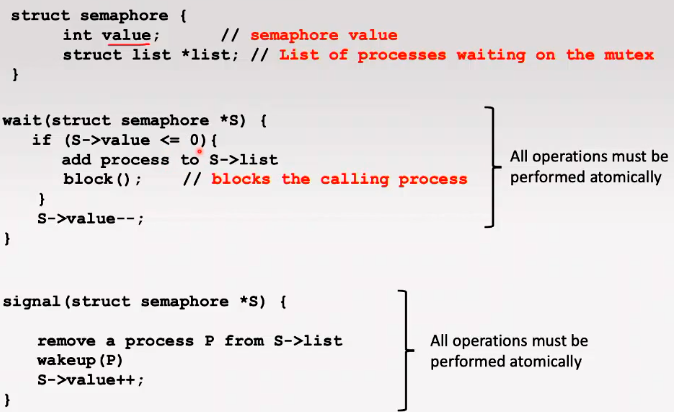
\includegraphics[width=0.8\textwidth]{fourtynine.png}
	\caption{Semaphore implementation}
	\label{fig:fourtynine-png}
\end{figure}
\end{tcolorbox}
\begin{tcolorbox}[colback=black!3!white,colframe=black!60!white,title=\begin{defn}Deadlock \label{Deadlock}\end{defn}]
Deadlock is when two or more processes waiting indefinitely for an event can only be caused by the waiting process. For example, $A$ waits for $B$ to do something. $B$ waits for $A$ to do something, therefore $A$ and $B$ are in deadlock. Let $S$ and $Q$ be two semaphores initialised to $1$.
\end{tcolorbox}
\begin{tcolorbox}[colback=black!3!white,colframe=black!60!white,title=\begin{defn}Starvation \label{Starvation}\end{defn}]
Starvation occurs when a specific process has to wait indefinitely whilst others make progress. Starvation occurs when multiple processes are waiting on a semaphore and the signal call wakes up the same process again and again. To avoid such starvation signal should randomly pick the process to wake up.
\end{tcolorbox}
\begin{tcolorbox}[colback=black!3!white,colframe=black!60!white,title=\begin{defn}Priority Inversion \label{Priority Inversion}\end{defn}]
Priority inversion is a scheduling problem when lower-priority process holds a lock needed by higher-priority process. It is solved via priority-inheritance protocol. Priority inheritance says that all processes that share the lock will share the same priority level. 
\end{tcolorbox}
\begin{tcolorbox}[colback=black!3!white,colframe=black!60!white,title=\begin{defn}Bounded Buffer Problem \label{Bounded Buffer Problem}\end{defn}]
This problem involves a buffer capable of storing $n$ items. Producer producers items and writes them to the buffer. The consumer consumers items from the buffer. We want to sync the producer and the consumer. There are three requirements
\begin{enumerate}
	\item Producer should not write when buffer is full
	\item Consumer should not read when buffer is empty
	\item Producer and consumer should not access the buffer at the same time
\end{enumerate}
Therefore, our code would be something like
\begin{figure}[H]
	\centering
	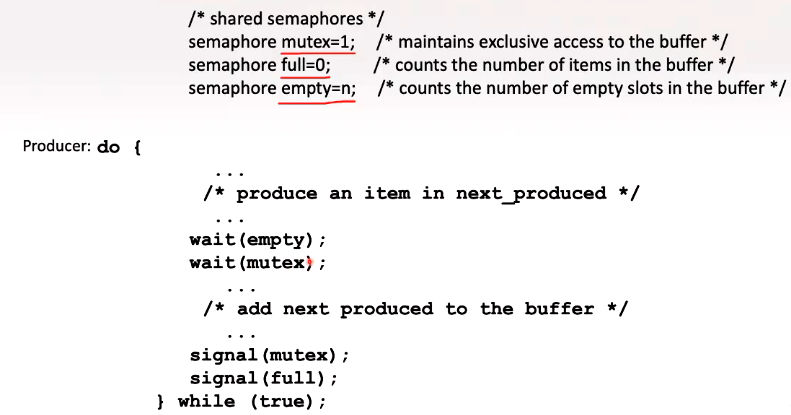
\includegraphics[width=0.8\textwidth]{fifty.png}
	\caption{Producer}
	\label{fig:fifty-png}
\end{figure}
\begin{figure}[H]
	\centering
	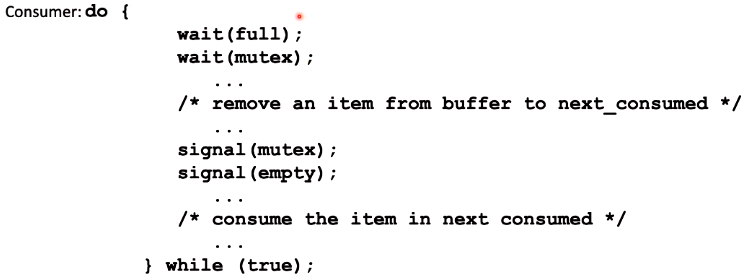
\includegraphics[width=0.8\textwidth]{fiftyone.png}
	\caption{Consumer}
	\label{fig:fiftyone-png}
\end{figure}
\end{tcolorbox}
\begin{tcolorbox}[colback=black!3!white,colframe=black!60!white,title=\begin{defn}Readers and Writers problem \label{Readers and Writers problem}\end{defn}]
A data set is shared among a number of concurrent processes. Readers only read the data set; they do not perform updates. Writers can both read and write. We want to allow multiple readers to read at the same time. However, only one single writer can access the shared data at the same time. There are many different versions involving different priorities. For our version, our readers are given preference over writers when no process is active. Writers may also starve. For the writer process we have
\begin{figure}[H]
	\centering
	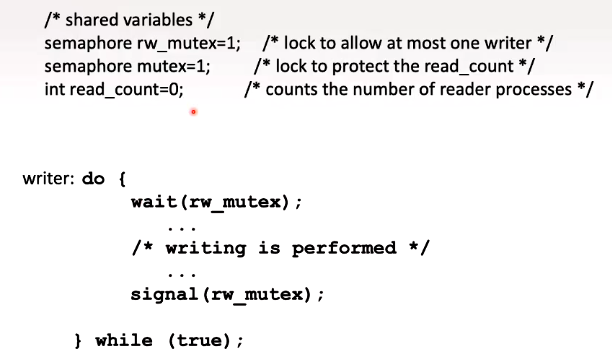
\includegraphics[width=0.8\textwidth]{fiftytwo.png}
	\caption{Writer Process}
	\label{fig:fiftytwo-png}
\end{figure}
And for the reader, we have
\begin{figure}[H]
	\centering
	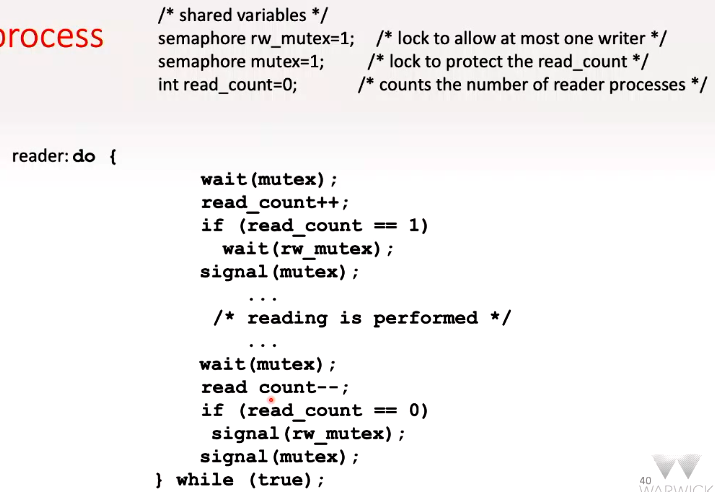
\includegraphics[width=0.8\textwidth]{fiftythree.png}
	\caption{Reader Process}
	\label{fig:fiftythree-png}
\end{figure}
\end{tcolorbox}
\begin{tcolorbox}[colback=black!3!white,colframe=black!60!white,title=\begin{defn}Dining Philosophers \label{Dining Philosophers}\end{defn}]
Philosophers spend their lives alternating thinking and eating. Don't interact wtih their neighbours, occasionally try to pick up $2$ chopsticks (one at a time) to eat from bowl. They need both to eat, and release both when done. In the case of $5$ philosophers, the shared data is the bowl of rice, the semaphore is the chopstick[5] all initialised to $1$ and two neighbouring philosophers cannot eat at the same time.
\begin{figure}[H]
	\centering
	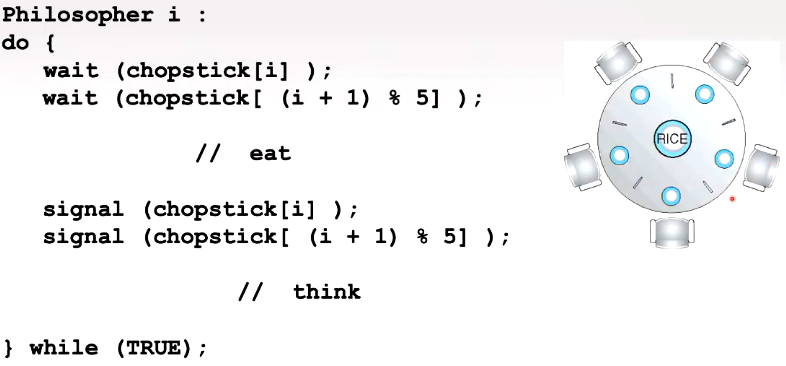
\includegraphics[width=0.8\textwidth]{fiftyfour.png}
	\caption{Dining Philosophers solution}
	\label{fig:fiftyfour-png}
\end{figure}
However, the solution above has a problem, where if all philosophers get hungry and they grab the left chopstick, they will be in a deadlock. There are however solutions to this. One way to fix is it is not to fill the table. For example, we allow at most 4 philosophers be sitting simultaneously at the table. We can also allow a philosopher to pick up the chopsticks only if both are available. Lastly, we can also use an asymmetric solution, use an odd-numbered philosopher picks up first the left chopstick and then the right chopstick. Even-numbered philosopher picks up the right chopstick and then the left chopstick
\end{tcolorbox}
\subsection{Deadlocks}
\begin{tcolorbox}[colback=black!3!white,colframe=black!60!white,title=\begin{defn}Deadlock \label{Deadlock}\end{defn}]
A set of processes is in a deadlock when each process in the set is waiting for an event that can be caused only by another process in the set. The event never occurs. The events we are interested in are acquisition or release of some type of resources, for example mutex locks, semaphores, cpu, file, i/o devices etc. 
\end{tcolorbox}
\begin{tcolorbox}[colback=black!3!white,colframe=black!60!white,title=\begin{exmp}A quick example \label{A quick example}\end{exmp}]
Given two processes $P_1$ and $P_2$ and two locks $L_1$ and $L_2$, we first have $L_1$ being acquired by $P_1$. Then, with context switch, we have $L_2$ is acquired by $P_2$. Then, through another context switch, we run $P_1$ again only to find that it is waiting for $L_2$. Similarly, with another context switch to $P_2$, we find that $P_2$ is waiting for $L_1$. If events occur in a different sequence, we may not see a deadlock. Therefore we have developed systematic methods to detect deadlocks.
\end{tcolorbox}
\begin{tcolorbox}[colback=black!3!white,colframe=black!60!white,title=\begin{defn}System Model \label{System Model}\end{defn}]
System consists of different types of resources $R_1,R_2,\ldots,R_m$ which are things such as mutex locks, CPUs, I/O devices etc. Each resource type $R_i$ has $W_i$ instances i.e., 3 mutex locks, 4 printers etc. A set of processes $\{P_0,P_1,\ldots,P_n\}$. Each process utilises a resource as follows: request, use, release.
\end{tcolorbox}
\begin{tcolorbox}[colback=black!3!white,colframe=black!60!white,title=\begin{defn}Necessary conditions for Deadlock \label{Necessary conditions for Deadlock}\end{defn}]
\begin{enumerate}
	\item Mutual Exclusion - only one process can use an instance of resource at a time
	\item Hold and Wait - there must be a process holding some resources while waiting to acquire additional resources held by other process
	\item No preemption - a resource can be released only voluntarily by the process holding it, after the process has completed its task
	\item Circular wait - there must exist $\{\overline{P}_0,\ldots,\overline{P}_m\} \subseteq \{P_0,\ldots,P_n\}$ such that $\overline{P}_0$ is waiting for $\overline{P}_1$, $\overline{P}_1$ is waiting for $\overline{P_2},\ldots,\overline{P}_m$ is waiting for $\overline{P}_0$
\end{enumerate}
\end{tcolorbox}
\begin{tcolorbox}[colback=black!3!white,colframe=black!60!white,title=\begin{defn}Resource Allocation Graph \label{Resource Allocation Graph}\end{defn}]
A directed graph $G=(V,E)$ where $V$ is partitioned into two types:
\begin{align*}
	P = \{P_1,P_2,\ldots,P_m\} & \text{the set consisting of all the processes in the system}\\
	R = \{R_1,R_2,\ldots,R_m\} & \text{the set consisting of all resource types in the system}
\end{align*}
The request edge is defined as the directed edge $P_i \to R_j$ \\
The assignment edge is defined as the directed edge $R_j \to  P_i$. \\
We will illustrate our graph using process nodes as circles and resource type nodes as squares with black dots in them which denote instances. For example, a square with $4$ black dots would denote a resource type with $4$ instances. 
\begin{figure}[H]
	\centering
	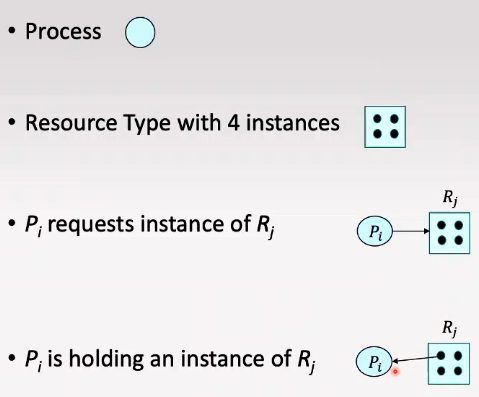
\includegraphics[width=0.5\textwidth]{sixtyseven.png}
	\caption{Illustration of our graph}
	\label{fig:sixtyseven-png}
\end{figure}
\end{tcolorbox}
\begin{tcolorbox}[colback=black!3!white,colframe=black!60!white,title=\begin{exmp}Resource Allocation Graph Example \label{Resource Allocation Graph Example}\end{exmp}]
        \begin{figure}[H]
        	\centering
        	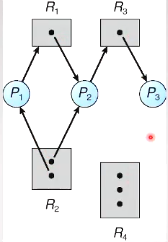
\includegraphics[width=0.3\textwidth]{sixtyeight.png}
        	\caption{Example Graph}
        	\label{fig:sixtyeight-png}
        \end{figure}
In the graph above, we have that $P_1$ has an instance of $R_2$ and has requested an instance from $R_1$. $P_2$ has instances of $R_1$ and $R_2$ but is waiting for instance of $R_3$. $P_3$ has instance of $R_3$. Is there a deadlock?\\
No. There are no cycles in the graph. Furthermore, even if there are smaller cycles in the graph, this does not indicated a deadlock. For a cycle to indicate a deadlock, none of the processes have all their requests satisfied.
\end{tcolorbox}
\begin{tcolorbox}[colback=black!3!white,colframe=black!60!white,title=\begin{defn}Conclusion for Graph \label{Conclusion for Graph}\end{defn}]
If graph contains no cycle $\implies$ no deadlock \\
If graph contains a cycle $\implies$ need to look further. For small examples, we can manually detect deadlocks. But for larger examples, we need an algorithm
\end{tcolorbox}
\begin{tcolorbox}[colback=black!3!white,colframe=black!60!white,title=\begin{defn}Deadlock Detecction Algorithm \label{Deadlock Detecction Algorithm}\end{defn}]
The algorithm involves transferring the graphical information into a tabular form. 
\begin{figure}[H]
	\centering
	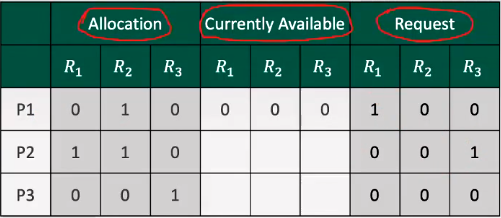
\includegraphics[width=0.6\textwidth]{sixtynine.png}
	\caption{Deadlock Detection Tabular Form}
	\label{fig:sixtynine-png}
\end{figure}
We further label that $P_1$, $P_2$ and $P_3$ are all unfinished, therefore their finish is false. However, we can set $P_3$ to true as it has no requests and reclaim the resource occupied for $R_3$. We can now satisfy $P_2$ request for $R_3$ and finish it as well. Lastly, we can finish $P_1$ now that we also have $R_1$ free.  
\end{tcolorbox}
\begin{tcolorbox}[colback=black!3!white,colframe=black!60!white,title=\begin{defn}Deadlock Prevention \label{Deadlock Prevention}\end{defn}]
We need to ensure that at least one of the necessary conditions for deadlocks does not hold. We cannot change the mutual exclusion rule, as it is required for some processes. Instead, we can modify the hold and wait rule, where we ensure a process either gets all or none of its required resources so it does not hold any other resources. We can also use no preemption, i.e., if a process holding some resources requests additional resources that cannot be immediately allocated to it, then all resources currently being held by the process can be released. Lastly, we can also modify circular wait. Number of resources and require that each process requests resources in an increasing order of enumeration. Process holding resource $n$ cannot request a resource with a number less than $n$.
\end{tcolorbox}
\begin{tcolorbox}[colback=black!3!white,colframe=black!60!white,title=\begin{defn}Deadlock Avoidance \label{Deadlock Avoidance}\end{defn}]
Deadlock avoidance is less restrictive than deadlock prevention. It determines if a request should be granted based on if the resulting allocation leaves the system in a safe state. Safe state is where deadlock can never occur, no matter what future requests arrive. We can determine if a state is safe using the deadlock avoidance algorithm. It needs a priori advanced information on resource requirements. Each process declares the maximum number of instances of each resource type that it may need. Upon receiving a resource request, the deadlock avoidance algorithm checks if granting the resource immediately leaves the system in a safe state. If so, grant the request immediately, otherwise wait until the state of the system changes to a state where the request can be granted safely. 
\end{tcolorbox}
\begin{tcolorbox}[colback=black!3!white,colframe=black!60!white,title=\begin{defn}Banker's Safety Algorithm \label{Banker's Safety Algorithm}\end{defn}]
Take 5 processes as an example denoted $P_0,\ldots,P_4$. There are 3 resource types, $A$, $B$ and $C$ which have $10$,$5$ and $7$ instances respectively. Consider the following table.
\begin{figure}[H]
	\centering
	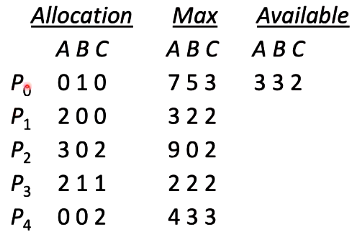
\includegraphics[width=0.4\textwidth]{seventy.png}
	\caption{Banker's Algorithm Table}
	\label{fig:seventy-png}
\end{figure}
Obtain additional need of each process, we do $max-allocation$. We can calculate $available = instances - \sum Allocation$. We now find processes whose additional needs satisfy currently available resources. For example, $P_1$ only needs $1\;2\;2$ which means that we can execute it. We will execute it and reclaim all the resources occupied by $P_1$. Therefore, we now have available $5\;3\;2$ resources. Next process we can satisfy is $P_3$ which now obtains us availability of $7\;4\;3$, continually until we have no processes left to execute. The order of sequence we have found is called a \textbf{safe sequence}. If a safe sequence exists, it means that the starting state of the system is safe.
\end{tcolorbox}
\begin{tcolorbox}[colback=black!3!white,colframe=black!60!white,title=\begin{defn}Resource Request Algorithm \label{Resource Request Algorithm}\end{defn}]
With Banker's safety algorithm we can determine if a given state is safe. However, to determine if a request for resource can be granted immediately, we need to determine if by granting the request we are in a safe state. Therefore, we have the resource request algorithm. Pretend the request is granted and determine if the resulting state is safe using Banker's safety algorithm. If it is found to be safe, we grant the request, otherwise we keep the request pending until state change.
\end{tcolorbox}
\subsection{Memory}
A program must be taken from disk into memory to be executed. Once in the memory, the process occupies some addresses which store instructions to run the process and data of input and output. The OS must allocate a unique set of addresses to each process. If not, then one process can modify data/instructions belonging to other processes. The OS must guarantee that a process is only able to access the addresses belonging to that process. During the execution of a process, the CPU needs to access different addresses belonging to the process. 
\begin{tcolorbox}[colback=black!3!white,colframe=black!60!white,title=\begin{defn}Logical vs Physical Address Space \label{Logical vs Physical Address Space}\end{defn}]
During the execution of a process, the CPU needs to access different addresses belonging to the process. Logical address generated by the CPU to fetch instructions or read/write data; may be different from actual physical address. The physical address is seen by the memory unit; a logical address must be converted to a physical address before a memory access. Lastly, MMU is special hardware, required to translate logical addresses to physical addresses.
\begin{figure}[H]
	\centering
	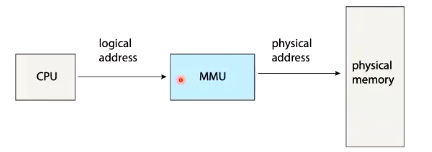
\includegraphics[width=0.8\textwidth]{seventyone.png}
	\caption{Logical to Physical}
	\label{fig:seventyone-png}
\end{figure}
The reason we separate logical and physical address is to make programming easier. The programmer does not need to worry about how the process is actually laid out in the memory.
\end{tcolorbox}
\begin{tcolorbox}[colback=black!3!white,colframe=black!60!white,title=\begin{defn}Memory Allocation \label{Memory Allocation}\end{defn}]
Memory allocation deals with how the OS allocates memory to processes and protects that memroy from other processes. We shall discuss three main techniques:
\begin{enumerate}
	\item Contiguous memory allocation
	\item Segmentation
	\item Paging
\end{enumerate}
\end{tcolorbox}
\begin{tcolorbox}[colback=black!3!white,colframe=black!60!white,title=\begin{defn}Contiguous Memory Allocation \label{Contiguous Memory Allocation}\end{defn}]
In contiguous memory allocation, each process is contained in a single section of memory starting from a base address. Each process occupies a contiguous block of addresses. This is a technique used in older OS's. To implement this scheme, the OS needs to decide the base address and the range of addresses for each process. The memory management unit (MMU) consists of relocation and limit registers storing the base address and range of addresses of a process. When a process is scheduled, the base and limit registers the loaded with the corresponding values by the OS. \\

Memory is divided into fixed size partitions. Each partitions is allocated to one process. When process terminates the partition is freed. There is a drawback, however, and that is the number of partitions in the memory fixes the number of concurrent processes in the memory. \\

In another case, where size partitions are variable. Any available block of memory is called a hole. Holes are scattered throughout memory. The OS keeps track of holes. When a process arrives, it is allocated memory from a hole large enough to accommodate it. Process exiting creates a hole, are combined into a single hole. 
\begin{figure}[H]
	\centering
	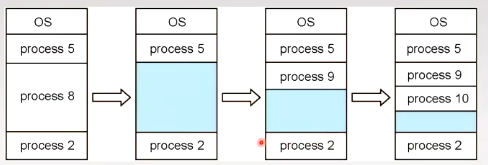
\includegraphics[width=0.7\textwidth]{seventytwo.png}
	\caption{Partitions and holes}
	\label{fig:seventytwo-png}
\end{figure}
However, the variable comes with an inherent problem: we need to track and allocate holes to incoming processes. The solutions are as follows:
\begin{itemize}
	\item First-fit - allocate the first hole that is big enough
	\item Best-fit - allocate the smallest hole that is big enough; must search entire list, unless ordered by size. It creates the smallest leftover hole
	\item Worst-fit - allocate the largest hole; must also search entire list. This produces the largest leftover hole. 
\end{itemize}
\end{tcolorbox}
\begin{tcolorbox}[colback=black!3!white,colframe=black!60!white,title=\begin{defn}Fragmentation \label{Fragmentation}\end{defn}]
Memory allocation method can fragment the usable memory space. Consider external fragmentation where the total memory space exists to satisfy a request, but it is not contiguous. Variable partitioning method suffers from this problem. Keeping tack of a large number of small holes may have a high overhead. \\
Another problem might be internal fragmentation. Allocated partition may be much larger than requested memory; this size difference is memory internal to a partition, but not being used  \\
In order to deal with the issue of fragmentation, we can use
\begin{itemize}
	\item Compaction - shuffle memory contents to place all free memory together in one contiguous block
	\item Non-contiguous memory allocation - allowing a process to be scattered throughout the memory
\end{itemize}
\end{tcolorbox}
\begin{tcolorbox}[colback=black!3!white,colframe=black!60!white,title=\begin{defn}Segmentation \label{Segmentation}\end{defn}]
For non-contiguous memory allocation, we divide a program into segments. Each segment is stored in a contiguous memory block. Each logical address consists of a two tuple
\begin{align*}
	<segment-number,offset>
\end{align*}
Segment number can be mapped to the base of the segment in the memory and offset is added to it to produce the complete physical address. \\
Segment table is indexed by segment numbers; each table entry has: segment-base and a segment-limit. The segment base contains where starting physical address where the segments reside in memory. The segment limit specifies the length of the segment
\end{tcolorbox}
\begin{tcolorbox}[colback=black!3!white,colframe=black!60!white,title=\begin{defn}Paging \label{Paging}\end{defn}]
Segmentation cannot avoid external fragmentation. We can instead avoid it with paging. We divide program into fixed-sized blocks called pages. We then divide physical memory into fixed-sized blocks called frames. We now have
\begin{align*}
	PageSize = FrameSize
\end{align*}
We then assign pages to frames. The mapping between page numbers and frame numbers is stored in a page table. For each process the OS maintains a separate page table. 
\end{tcolorbox}
\begin{tcolorbox}[colback=black!3!white,colframe=black!60!white,title=\begin{defn}Logical Address under Paging \label{Logical Address under Paging}\end{defn}]
Address generated by CPU is divided into
\begin{itemize}
	\item Page number ($p$) - used as an index into a page table which contains base address of each page in physical memroy
	\item Page offset ($d$) - combined with base address to define the physical memory address that is sent to the memory unit.
\end{itemize}
If logical address is $m$ bits and pages size is $2^{n}$ bytes then last $n$ bits is used to denote the page offset.
\begin{figure}[H]
	\centering
	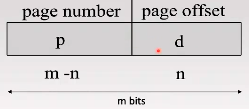
\includegraphics[width=0.3\textwidth]{seventythree.png}
	\caption{Table breakdown}
	\label{fig:seventythree-png}
\end{figure}
In the figure below, observe how address is retrieved: the $p$ is indexed in the page table to obtain the frame address $f$. It is then concatenated with the number from $d$, which is the logical address.
\begin{figure}[H]
	\centering
	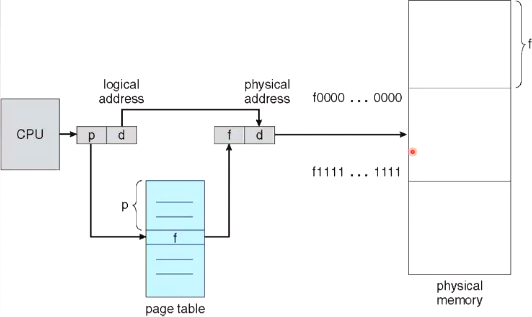
\includegraphics[width=0.7\textwidth]{seventyfour.png}
	\caption{Paging Retrieval}
	\label{fig:seventyfour-png}
\end{figure}
Notice that internal fragmentation cannot occur as we divide frames and pages perfectly. Except, however, the last leftover frame with remainder bytes will be the only wasted bytes. 
\end{tcolorbox}
We will now discuss how page translation is implemented in an OS using hardware.
\begin{tcolorbox}[colback=black!3!white,colframe=black!60!white,title=\begin{defn}Directly from the memory \label{Directly from the memory}\end{defn}]
When a CPU generates page number and offset address for a process, we will use that page number to index into the page table. The page table itself is stored in the memory, therefore we need to locate the page table. We need to store the base address of a page table in the PCB. When a process is scheduled the base address of the page table is loaded into a register called page table base register (PTBR). Page number is added to the base address to find the location in memory where the corresponding frame number is stored.
\begin{figure}[H]
	\centering
	\includegraphics[width=0.8\textwidth]{seventyfive.png}
	\caption{Illustration}
	\label{fig:seventyfive-png}
\end{figure}
The drawback is that at least two memory accesses are required to fetch every instruction/data, increasing overhead.
\end{tcolorbox}
\begin{tcolorbox}[colback=black!3!white,colframe=black!60!white,title=\begin{defn}Translation Lookaside Buffer (TLB) \label{Translation Lookaside Buffer (TLB)}\end{defn}]
Translation lookaside buffer is a hardware cache to store frequently used page table entries. It stores a small number of entries, $<256$. When the CPU generates a logical address its page number is checked against all the entries in TLB in parallel to find a match. 
\begin{figure}[H]
	\centering
	\includegraphics[width=0.8\textwidth]{seventysix.png}
	\caption{TLB}
	\label{fig:seventysix-png}
\end{figure}
TLB is small and is cache memory, therefore the search is really fast. If TLB misses, then we try to find our page using the page table. We then fill the TLB with that specific entry we were looking for in case for the future. The TLB can store page table entries of multiple processes. However, each entry of the TLB requires an address space identifier (ASID) to uniquely identify the process requesting the TLB search. If ASIDs match, then the frame number is returned; otherwise the request is considered to be a cache miss, which also guarantees memory protection. 
\end{tcolorbox}
\begin{tcolorbox}[colback=black!3!white,colframe=black!60!white,title=\begin{defn}Effective Access Time \label{Effective Access Time}\end{defn}]
The effective access time is defined as the following
\begin{align}
\text{Effective Access Time} = \text{Hit Ratio} \times  1 \times \text{Memory Access} + \left( 1-\text{Hit ratio} \right) \times 2\times \text{Memory Access}
\end{align}
\end{tcolorbox}
\begin{tcolorbox}[colback=black!3!white,colframe=black!60!white,title=\begin{exmp}Access Time Example \label{Access Time Example}\end{exmp}]
        Given a $95\%$ hit ratio and a $100$ ns access time, what is the effective access time? We have
	\begin{align*}
		EAT &= 0.95 \times 100 + 0.05 \times 200\\
	&= 105\text{ns}
	\end{align*}
\end{tcolorbox}
\begin{tcolorbox}[colback=black!3!white,colframe=black!60!white,title=\begin{defn}Smaller Page Tables \label{Smaller Page Tables}\end{defn}]
It is beneficial to have small page tables, it helps us reduce the memory overhead and reduce the page search time in case of a TLB miss. Most modern systems use $32$ or $64$ bit logical addresses. With $32$ bit addresses and a $4$ KB page size, the number of entries is $2^{20}$. If each entry requires $4$ bytes, then the size of a page table is $4$ MB. Imagine the memory overhead if we are to run $100$ processes. 
\end{tcolorbox}
\begin{tcolorbox}[colback=black!3!white,colframe=black!60!white,title=\begin{defn}Hierarchal Multi-level paging tables \label{Hierarchal Multi-level paging tables}\end{defn}]
We divide the page table into pages and store each page in a frame in the memory. That is, we store different pages in pages, compressing our original paging table. However, we will have to store an outer page table to store our newly created pages that map to our original pages. If the outer page table is bigger than one frame, we can further divide it into pages. The OS does not need to store the inner PTs not in use. The flat page requires $4$ MB of space which is larger than $4$ KB that is the page size. To store the inner page tables we would need $2^{10}=\frac{4MB}{4KB}$ frames. The outer page table will therefore have $2^{10}$ entries of $4$ bytes each. Total size is $4$ KB. Fits into one frame. No further paging required. Then, addressing is know defined as follows:
\begin{figure}[H]
	\centering
	\includegraphics[width=0.6\textwidth]{seventyseven.png}
	\caption{Addressing with Multi-Level Paging}
	\label{fig:seventyseven-png}
\end{figure}
However, now we have 3 memory accesses instead of $2$. Multi-Level paging reduces the memory overhead but increases the number of memory accesses required to read/write data in case of a TLB miss. 
\end{tcolorbox}
\begin{tcolorbox}[colback=black!3!white,colframe=black!60!white,title=\begin{defn}Hashed Table Maps \label{Hashed Table Maps}\end{defn}]
Page numbers serve as hash keys and are hashed at an index of the PT. Each entry is a pointer to a linked list of page numbers having the same hash value. Each node contains the page number, the frame number and a pointer to the next node. Page numbers are compared in this chain searching for a match. If a match is found, the corresponding physical frame is extracted.
\end{tcolorbox}
\section{Networks}
\subsection{Components of a network}

	\begin{tcolorbox}[colback=black!3!white,colframe=black!60!white,title=\begin{defn}Network \label{Network}\end{defn}]
	A network of inter-connected computing devices which enable processes running on different devices to communicate. Processes communicate by sending messages. Intermediate nodes help forward messages. For example, the internet.
	\end{tcolorbox}
\begin{tcolorbox}[colback=black!3!white,colframe=black!60!white,title=\begin{defn}Network Edge \label{Network Edge}\end{defn}]
Consists of end hosts which run network applications, e.g., Web, Email, Video Streaming, Online games.
\end{tcolorbox}
\begin{tcolorbox}[colback=black!3!white,colframe=black!60!white,title=\begin{defn}Network core \label{Network core}\end{defn}]
consists of packet switches which help forward data packets e.g., switch and router
\end{tcolorbox}
\begin{tcolorbox}[colback=black!3!white,colframe=black!60!white,title=\begin{defn}Communication links \label{Communication links}\end{defn}]
carry data between network devices as electromagnetic waves. E.g., fiber, copper, radio, satellite links
\end{tcolorbox}
\begin{figure}[H]
	\centering
	\includegraphics[width=0.8\textwidth]{sixteen.png}
	\caption{Components of a network}
	\label{fig:sixteen-png}
\end{figure}
\begin{tcolorbox}[colback=black!3!white,colframe=black!60!white,title=\begin{defn}End-host \label{End-host}\end{defn}]
End-hosts run application processes e.g., mail, web which generate messages. It breaks down application messages into smaller chunks called packets. It adds additional information e.g., IP address, port number as packet headers so that the packets can be carried by the internet to their destinations. The IP address uniquely identifies an end host in the network and a port number uniquely identifies a process running within an end host. It then sends these bits over a physical medium. If needed provides reliable and orderly delivery of the packets. It also controls the rate of transmissions of packets
\end{tcolorbox}
\begin{tcolorbox}[colback=black!3!white,colframe=black!60!white,title=\begin{defn}Network Core \label{Network Core}\end{defn}]
The network core has a function of routing - run routing algorithms to construct routing tables. It also has a function of forwarding - once a packet arrives, it is forwarded to the appropriate output link according to the routing table.
\subsection{Delay}
\begin{figure}[H]
	\centering
	\includegraphics[width=0.8\textwidth]{seventeen.png}
	\caption{Routing}
	\label{fig:seventeen-png}
\end{figure}
\end{tcolorbox}
\begin{tcolorbox}[colback=black!3!white,colframe=black!60!white,title=\begin{defn}Store-and-forward principle \label{Store-and-forward principle}\end{defn}]
\begin{figure}[H]
	\centering
	\includegraphics[width=0.8\textwidth]{eighteen.png}
	\caption{Store-and-forward principle}
	\label{fig:eighteen-png}
\end{figure}
The store and forward principle consists of the idea that an entire packet must arrive at router before it can be transmitted on next link. It takes $\frac{L}{R}$ seconds to transmit $L $-bit packet into link at $R$ bps. The end-to-end delay is  $\frac{2L}{R}$.
\end{tcolorbox}
\begin{tcolorbox}[colback=black!3!white,colframe=black!60!white,title=\begin{defn}Queueing delay and loss \label{Queueing delay and loss}\end{defn}]
If arrival rate (in bits) to link exceeds transmission rate of link for a period of time, packets will be in queue waiting to be transmitted on link or packets can be dropped (lost) if memory fills up.
\begin{figure}[H]
	\centering
	\includegraphics[width=0.8\textwidth]{nineteen.png}
	\caption{Queueing delay}
	\label{fig:nineteen-png}
\end{figure}
\end{tcolorbox}
\begin{tcolorbox}[colback=black!3!white,colframe=black!60!white,title=\begin{thm}Four sources of delay \label{Four sourceso f delay}\end{thm}]
	There are sources of delay:
	\begin{enumerate}
		\item $d_{trans}$ - transition delay - $d_{trans} = \frac{L}{R}$- where $L$ is packet length (bits) and $R$ is link bandwidth (bps)
		\item $d_{queue}$ - queueing delay - time waiting at output link for transmission (depends on congestion level of router)
		\item $d_{proc}$ - nodal processing - checks bit errors, determines output link and typically $<msec$
		\item $d_{prop}$ - propagation delay - $d_{prop} = \frac{d}{s}$ - where $d$ is length of physical link and $s$ is propagation speed in medium (approx $2\times 10^{8}\frac{m}{s}$ )
	\end{enumerate}
	The final formula is
		\begin{align}
		d_{nodal} = d_{proc}+d_{queue}+d_{trans}+d_{prop}
		\end{align}
		\begin{figure}[H]
			\centering
			\includegraphics[width=0.6\textwidth]{twenty.png}
			\caption{Delay process}
			\label{fig:}
		\end{figure}
\end{tcolorbox}
Ty\begin{tcolorbox}[colback=black!3!white,colframe=black!60!white,title=\begin{defn}Throughput \label{Throughput}\end{defn}]
Throughput is specific to flow or communicating pair. It is the rate at which bits are transferred from src to dest in a given time window $\frac{\text{bits}}{\text{time}}$. It can be either instantaneous (rate at given point in time) or average (rate over longer period of time). 
\end{tcolorbox}
\subsection{Internet}

\begin{tcolorbox}[colback=black!3!white,colframe=black!60!white,title=\begin{defn}Protocol \label{Protocol}\end{defn}]
Communicating nodes must agree on certain rules. A protocol define format, order of msgs sent out and received among network entities, and actions taken on msg transmission, receipt. Network protocols can be implemented either as software or as hardware.
\end{tcolorbox}
\begin{tcolorbox}[colback=black!3!white,colframe=black!60!white,title=\begin{defn}Packet Switching \label{Packet Switching}\end{defn}]
The internet uses packet switching technology. Different flows (source-dest pairs) share resources (links) along their routes. Internet traffic is bursty in nature. If one flow is not using a link, then other flows can use it. Flows can change routes if link fails or becomes congested.
\end{tcolorbox}
\begin{tcolorbox}[colback=black!3!white,colframe=black!60!white,title=\begin{defn}Circuit Switching \label{Circuit Switching}\end{defn}]
Before the internet, circuit switching was used in telephone networks. A circuit consists of all communication links and nodes along a path from source to destination. In circuit switching, a circuit is reserved for each flow for the entire call duration. Guaranteed rate of communication. Flows do not share resources. If one flow is not using its assigned circuit during the call, it cannot be used by another flow. Not ideal for bursty internet traffic. If link fails, call must end.
\end{tcolorbox}
\begin{figure}[H]
	\centering
	\includegraphics[width=0.8\textwidth]{twentyone.png}
	\caption{Packet vs Circuit}
	\label{fig:twentyone-png}
\end{figure}		
\begin{tcolorbox}[colback=black!3!white,colframe=black!60!white,title=\begin{defn}Design Philosophy Layering \label{Design Philosophy Layering}\end{defn}]
Network devices perform complex function. It is better to divide the functions into "layers". Each layer performs a subset of functions. Layer $N$ uses the services of Layer $N-1$ and provides services to Layer $N+1$. Layering makes it easier to add services to a layer or change its implementation without affecting other layers. The internet protocol stack has 5 layers containing all possible functions.
\begin{figure}[H]
	\centering
	\includegraphics[width=0.2\textwidth]{twentytwo.png}
	\caption{Internet Protocol Stack}
	\label{fig:twentytwo-png}
\end{figure}
\begin{figure}[H]
	\centering
	\includegraphics[width=0.8\textwidth]{twentythree.png}
	\caption{Internet Protocol Stack}
	\label{fig:twentythree-png}
\end{figure}
\end{tcolorbox}
\begin{tcolorbox}[colback=black!3!white,colframe=black!60!white,title=\begin{defn}Sockets \label{Sockets}\end{defn}]
Sockets are APIs between the application and transport layers. It is analogous to doors. Whenever the sender has a message to send, it creates a socket and writes message onto the socket with proper addressing info. The layers below and the internet is responsible for carrying the message to the receiving process. The receiver has another socket into which the message is written. The receiving process simply reads the message from the socket.
\begin{figure}[H]
	\centering
	\includegraphics[width=0.8\textwidth]{twentyfour.png}
	\caption{Socket, internet and user process functionality}
	\label{fig:twentyfour-png}
\end{figure}
\end{tcolorbox}
\begin{tcolorbox}[colback=black!3!white,colframe=black!60!white,title=\begin{defn}Addressing Processes \label{Addressing Processes}\end{defn}]
Messages need to be addressed to the correct process running within the correct end host. Any internet devices can be identified by its IP address. IPv4 addresses are $32$ bit numbers written as dotted decimal e.g., 154.31.16.13. Processes can be identified by port numbers. Port numbers are $16$ bit numbers ranging from $0$ to $2^{16}-1$. Port numbers $0$ to $1023$ are reserved for well known network applications e.g., $80$ for \mathbb{H}TP. Port numbers above $1023$ can be used by other application programmes.
\end{tcolorbox}
\subsection{Transport Layer}
Transport layers are used by application processes to deliver messages to their intended recipients. All transport layer protocols offer some basic services. For example, packetisation, addresing, sequencing, error correcting bits. An app may require additional services from the transport layer, such as reliable and in-order delivery of packets.
\begin{tcolorbox}[colback=black!3!white,colframe=black!60!white,title=\begin{defn}Transmission Control Protocol (TCP) \label{Transmission Control Protocol (TCP)}\end{defn}]
The TCP offers reliable and in-order data transfer service: packets can be lost or arrive out of order. It also provides connection oriented service: setup required between client and server processes before they start transferring data, called TCP handshake.
\begin{figure}[H]
	\centering
	\includegraphics[width=0.6\textwidth]{twentyfive.png}
	\caption{TCP protocol}
	\label{fig:twentyfive-png}
\end{figure}
For example, HTTP uses port 80 and TCP to run. In HTML 1.0, TCP was used separately for every single file found on the server, meaning that there were multiple handshakes causing delay. In 1.1, a single TCP can send multiple files. \\

TCP also incorporates flow control i.e., it matches the sending speed of the sender to the reading speed of the receiver. It further provides congestion control.
\end{tcolorbox}
\begin{tcolorbox}[colback=black!3!white,colframe=black!60!white,title=\begin{defn}User Datagram Protocol (UDP) \label{User Datagram Protocol (UDP)}\end{defn}]
UDP provides no guarantees on data transfer. UDP however, is really fast. No connection setup is required, UDP headers are smaller than TCP headers. There is also no effort made to recover losses. UDP is connection-lesss : each UDP segment is treated independently. Furthermore, UDP offers no congestion control. Using UDP, senders can send at any rate they wish even when the network is congested. Despite these, we use UDP mainly because it is fast and it has less overhead. Having no connection establishment (handshaking), meaning that there is less delay. It has smaller header size than TCP. There is no congestion control: UDP sender can blast away as fast as desired such as video streaming, internet telephony etc. Because the transport layer does not have reliability, we instead build the reliability at the application layer. 
\end{tcolorbox}
\begin{tcolorbox}[colback=black!3!white,colframe=black!60!white,title=\begin{exmp}Non-Persistent HTTP \label{Non-Persistent HTTP}\end{exmp}]
        \begin{enumerate}
        	\item The client sends SYN, the server responds with SYN-ACK
		\item Client sends ACK and adds request for the base HTML file
		\item The server establishes the connection and responds with the base HTML file
		\item HTTP server closes TCP connection
		\item Client receives the HTML file and examines it to find $10$ other references objects
		\item Steps $1-4$ are repeated for each of the $10$ objects
        \end{enumerate}
	\begin{figure}[H]
		\centering
		\includegraphics[width=0.5\textwidth]{twentysix.png}
		\caption{RTT}
		\label{fig:twentysix-png}
	\end{figure}
	We use $1$ RTT (round trip time) to initiate TCP connection. $1$ RTT to send HTTP request and receive first bytes of the requested object. There is also transmission time, meaning
	\begin{align*}
		\text{Response Time}=2\text{RTT}+\text{File transmission time}
	\end{align*}
	Each object requires at least $2 $RTT to be downloaded. For each TCP connection, the OS of the server has to allocate some resources e.g., buffers, local variables etc. Problematic when the server has to handle a large number of requests.
\end{tcolorbox}
\begin{tcolorbox}[colback=black!3!white,colframe=black!60!white,title=\begin{exmp}Persistent HTTP \label{Persistent HTTP}\end{exmp}]
        \begin{enumerate}
        	\item The server leaves connection open after sending response
		\item Subsequent HTTP messages are exchanged over open connection
		\item Client sends request back-to-back as soon as it encounters a references object
		\item All objects can be downloaded within $2 $RTT+ total data transfer time
        \end{enumerate}
\end{tcolorbox}
\begin{tcolorbox}[colback=black!3!white,colframe=black!60!white,title=\begin{defn}Web Cache \label{Web Cache}\end{defn}]
The goal of a web cache is to satisfy client request without involving origin server. Web clients can be configured to access the web via a web cache. Browser sends all HTTP requests to cache. Objects in cache returns the object and if cache request object from origin server, then returns object to client. The idea is that it reduces response time for client request. It also reduces traffic going out of an ISP network. Reduces the cost for the ISP. Lastly, it reduces the traffic on the internet as a whole.
\end{tcolorbox}
\subsection{Selected Topics in Networking}
\begin{tcolorbox}[colback=black!3!white,colframe=black!60!white,title=\begin{defn}Network Interface \label{Network Interface}\end{defn}]
A network interface is the point of interconnection between a computer/device and a network. A network interface is typically associated with a hardware network interface card (NIC). Each network in the internet has an IP address. Interfaces associated to hardware NIC also have a hardware address or a MAC address. 
\end{tcolorbox}
\begin{tcolorbox}[colback=black!3!white,colframe=black!60!white,title=\begin{defn}SYN attack \label{SYN attack}\end{defn}]
In a SYN attack, the attacker sends a lot of SYN requests at once. In most cases, they're sent from spoofed IP addresses. The TCP server then responds by creating half-open connections for each request, using a lot of resources. After sending back SYN-ACK packets, the attacker will not respond and the server will have to keep these packets open for a specific period, causing a jam. 
\end{tcolorbox}
\begin{tcolorbox}[colback=black!3!white,colframe=black!60!white,title=\begin{defn}ARP Cache Poisoning Attack \label{ARP Cache Poisoning Attack}\end{defn}]
To understand this attack we need to understand how MAC addresses and what the address resolution protocol (ARP) is. \\

A MAC changes as a packet travels. For example, 
\begin{figure}[H]
	\centering
	\includegraphics[width=0.8\textwidth]{thirtyfour.png}
	\caption{MAC Address in networks}
	\label{fig:thirtyfour-png}
\end{figure}
In the above figure, we can see that the network header describes from which IP the packet is sent to, and its destination IP. However, in the link header, we will have a source mac address and destination mac address, which is more local. In other words, if a packet travels from A to B, it first requires to travel from the device to the first router entrance MAC address. Once the first node, the mac address source and destination change once more, i.e.,
\begin{figure}[H]
	\centering
	\includegraphics[width=0.4\textwidth]{thirtyfive.png}
	\caption{New MAC src and dest}
	\label{fig:thirtyfive-png}
\end{figure}
However, we now need to know which new mac address to send it to. This is resolved by the address resolution protocol (ARP). This is done by using the destination IP address. The router will run its own routing algorithm to determine the next destination, specifically, which IP address it should hop into to reach its destination. Once the target is found, the router runs ARP to map the found IP address to a MAC address. The ARP sends an ARP request message to all the devices connected to that router with a specific broadcasting mac address. Only the router with the corresponding IP address will respond to this message. Once the reply is received, it stores the MAC address in the router's cache. ARP allows unsolicited replies since IP addresses can change. An attacn send an unsolicited ARP reply pretending to be someone else.
\end{tcolorbox}
\subsection{Transport Layer 2}
Transport layer provides logical communication between app processes running on different hosts. Transport protocols run in end systems. There is the send side, which breaks app messages into segments, adds header and passes to network layer. There is also the receive side, which reassembles segments into messages and passes it to the app layer. See TCP and UDP for a refresh.

\begin{tcolorbox}[colback=black!3!white,colframe=black!60!white,title=\begin{defn}Reliable transfer over a unreliable channel \label{Reliable transfer over a unreliable channel}\end{defn}]
We need to understand the general requirements for building reliable data transfer over an unreliable channel. In an unreliable channel there can be bit errors due to electrical noise, loss packets due to buffer overflow and packets can arrive in wrong order due to different delays of channels. Therefore, in the headers we implement
\begin{itemize}
	\item Checksums - to detect errors. Include the sum of all 16-bit words in the header.
	\item Acknowledgements or ACKs - to indicate if a packet is correctly received at the receiver. 
	\item Timeout mechanism - sender times out if ACK is not received within a timeout interval
	\item Retransmissions - to retransmit lost or corrupted packets. Automatic Repeat Request (ARQ)
	\item Sequence Number - to correctly order packets 
\end{itemize}
\end{tcolorbox}
\begin{tcolorbox}[colback=black!3!white,colframe=black!60!white,title=\begin{defn}Stop and Wait ARQ \label{Stop and Wait ARQ}\end{defn}]
In stop and wait ARQ, the sender sends a packet and waits until it receives ACK. If ack arrives, sends the next packet else times out and retransmits the same packet.
\begin{figure}[H]
	\centering
	\includegraphics[width=0.8\textwidth]{fiftyfive.png}
	\caption{Stop and wait ARQ}
	\label{fig:fiftyfive-png}
\end{figure}
\end{tcolorbox}
\begin{tcolorbox}[colback=black!3!white,colframe=black!60!white,title=\begin{exmp}Performance of stop and wait ERQ \label{Performance of stop and wait ERQ}\end{exmp}]
        Suppose we have a $1$ Gbps link $R=10^{9}$ bps. Packet length is $L = 8000$ bits. 
	\begin{figure}[H]
		\centering
		\includegraphics[width=0.5\textwidth]{fiftysix.png}
		\caption{Problem in an image}
		\label{fig:fiftysix-png}
	\end{figure}
	The utilisation $U$ is then calculated by
	\begin{align*}
		U = \frac{\frac{L}{R}}{RTT+\frac{L}{R}}= \frac{L}{R \times RTT + L} = 0.00027
	\end{align*}
	which, for window based pipelined protocols are
	\begin{align*}
		U = \frac{min\left( B,L+R\times RTT\right) }{L+R\times RTT}
	\end{align*}
\end{tcolorbox}
\begin{tcolorbox}[colback=black!3!white,colframe=black!60!white,title=\begin{defn}Delay Bandwidth Product \label{Delay Bandwidth Product}\end{defn}]
Sender should be allowed to send more packets without waiting for the ACK. Sender could send $R \times  RTT$ bits of additional data during the $RTT$ interval. Furthermore, for the length of pipeline defined as $L+R\times RTT$ with buffer size $B$ bits, we have that the maximum number of bits without waiting for ACK is
\begin{align*}
	min(B,L+R\times RTT)
\end{align*}
\end{tcolorbox}
\begin{tcolorbox}[colback=black!3!white,colframe=black!60!white,title=\begin{defn}Pipelined protocols \label{Pipelined protocols}\end{defn}]
Pipelined protocols allow multiple unacknowledged packets in the pipeline. ACK is sent individually or cumulatively. Range of sequence numbers must be increased. There are two generic protocols called Go-Back-N and Selective Repeat. 
\end{tcolorbox}
\begin{tcolorbox}[colback=black!3!white,colframe=black!60!white,title=\begin{defn}Go-Back-N Protocol \label{Go-Back-N Protocol}\end{defn}]
In the Go-Back-N protocol, the sender can send up to $N$ packets without waiting for ACK. $N$ is the window size, depends on the delay-bandwidth product, receive buffer size. The receiver maintains a variable $expectedseqnum$ which keeps track of the next expected sequence number to be received. If the receiver correctly receives packet $n$ and $n=expectedseqnum$ then it sends $ACK(n)$ which acknowledges all packets up to including packet $n$. This is called cumulative ack. In the case of $n \neq expectedseqnum$, the receiver discards the incoming packet and sends $ACK(expectedseqnum-1)$ 
\begin{figure}[H]
	\centering
	\includegraphics[width=0.8\textwidth]{fiftyseven.png}
	\caption{Go-Back-N Visualised}
	\label{fig:fiftyseven-png}
\end{figure}
\begin{figure}[H]
	\centering
	\includegraphics[width=0.8\textwidth]{fiftyeight.png}
	\caption{Go-Back-N Scenario $2$ Visualised}
	\label{fig:fiftyeight-png}
\end{figure}
\end{tcolorbox}
\begin{tcolorbox}[colback=black!3!white,colframe=black!60!white,title=\begin{defn}Selective Repeat (SR) \label{Selective Repeat (SR)}\end{defn}]
The SR receiver does not discard out of order packets, as long as they fall inside the receive window. The receiver has a window size $N$ which is the same size as the send window $N$. ACKs are also not cumulative but are individual, meaning that each packet gets acknowledged individually. The sender maintains a timer for each unacked packet in its send window. If the timer runs out, the sender sends that specific timed out packet again. The SR sender does not have to retransmit out-of-order packets. 
\begin{figure}[H]
	\centering
	\includegraphics[width=0.8\textwidth]{fiftynine.png}
	\caption{Selective Repeat}
	\label{fig:fiftynine-png}
\end{figure}
\begin{figure}[H]
	\centering
	\includegraphics[width=0.8\textwidth]{sixty.png}
	\caption{SR in action}
	\label{fig:sixty-png}
\end{figure}
\end{tcolorbox}
\begin{tcolorbox}[colback=black!3!white,colframe=black!60!white,breakable,enhanced,title=\begin{defn}TCP reliable data transfer \label{TCP reliable data transfer}\end{defn}]
TCP uses a combination of GBN and SR protocols. Like GBN, TCP uses cumulative ACKs and like SR, the TCP sender only retransmits the segment causing timeout. To understand how TCP works, we first need to understand how sequence numbers are assigned to packets. In TCP, each byte of data is numbered. Sequence number of a transmitted TCP segment is the "byte" number of the first byte of the segment. TCP ACK is the number of next expected byte from the other side. TCP uses cumulative ACKs. In TCP, data can flow in both directions. To reduce the number of transmissions, TCP piggybacks ACKs on data segments. A segment can carry data and serve as an ACK. 
\begin{figure}[H]
	\centering
	\includegraphics[width=0.4\textwidth]{sixtyone.png}
	\caption{Lost ACK Scenario}
	\label{fig:sixtyone-png}
\end{figure}
\begin{figure}[H]
	\centering
	\includegraphics[width=0.3\textwidth]{sixtytwo.png}
	\caption{Delayed ACK scenario}
	\label{fig:sixtytwo-png}
\end{figure}
\begin{figure}[H]
	\centering
	\includegraphics[width=0.4\textwidth]{sixtythree.png}
	\caption{Cumulative ACK Scenario}
	\label{fig:sixtythree-png}
\end{figure}
\begin{figure}[H]
	\centering
	\includegraphics[width=0.4\textwidth]{sixtyfour.png}
	\caption{Lost Packet Scenario}
	\label{fig:sixtyfour-png}
\end{figure}
The time-out period is often relatively long. Long delay before resending lost packet. TCP fast transmit means that duplicate ACKs are a good indicators of packet loss. They are sent when there is a gap in the received stream of bytes. It allows for faster re-transmit of the lost packet instead of waiting for the timeout period.
\end{tcolorbox}
\begin{tcolorbox}[colback=black!3!white,colframe=black!60!white,title=\begin{defn}Flow Control \label{Flow Control}\end{defn}]
The data in the pipeline should not exceed the receive buffer size. Otherwise, the receive buffer will overflow and data will be lost. Flow control tries to adjust the sending speed of the sender according to the space available at the buffer. Receiver advertises the free buffer space in the receive window field. It is denoted by rwnd. Sender limits amount of unacked "in-flight" data to receiver's $rwnd$ value.
\begin{align*}
	W = LastByteSent - LastByteAcked \le rwnd
\end{align*}
This guarantees receive buffer will not overflow
\end{tcolorbox}
\begin{tcolorbox}[colback=black!3!white,colframe=black!60!white,title=\begin{defn}Congestion Control \label{Congestion Control}\end{defn}]
Reliable data transfer and flow control are directly beneficial to the applications. TCP provides congestion control which is beneficial for the network as a whole. It controls the rate of transmission according to the level of perceived congestion. \\
Congestion at a router occurs when $inputRate > outputRate$. The manifestations include lost packets due to buffer overflow at routers or long delays for queueing in router buffers. The key cause of a congestion in a network are senders sending packets too fast. The goal of congestion control is to control the rate of the senders such that congestion does not occur in the network and that each flow gets a fair share of network resources. A TCP sender assumes the network to be congested when
\begin{enumerate}
	\item Timeout occurs
	\item Three duplicate ACKs are received
\end{enumerate}
TCP treats these events differently. A timeout event is taken more seriously than the reception of $3$ duplicate ACKs. If window size is $W$ bytes, the rate of transmission is approximately
\begin{align*}
	\frac{W}{RTT}
\end{align*}
Controlling $W$ controls the transmission rate. The maximum size of a TCP segment is called the Maximum Segment Size (MSS). The number of segments to transmit all data in the window is
\begin{align*}
	 \left|\frac{W}{MSS}\right|
\end{align*}
Sender maintains the congestion window size denoted by $cwnd$ and 
\begin{align*}
	W = LastByteSent - LastByteAcked \le min\left( cwnd,rwnd \right) 
\end{align*}
$cwnd$ is dynamic, function of perceived network congestion. It is calculated by the idea that the sender linearly increases transmission rate (cwnd) until loss occurs. If loss occurs  reduce he rate by a factor of $2$. Additive increase: $cwnd$ by $1 $ MSS every RTT until loss is detected. There is also multiplicative decrease where we cut $cwnd$ in half after loss. 
\begin{figure}[H]
	\centering
	\includegraphics[width=0.8\textwidth]{sixtyfive.png}
	\caption{AIMD}
	\label{fig:sixtyfive-png}
\end{figure}	
This allows fair rate allocation among competing flows.
\end{tcolorbox}
\begin{tcolorbox}[colback=black!3!white,colframe=black!60!white,title=\begin{defn}TCP Slow Start and ssthresh \label{TCP Slow Start and ssthresh}\end{defn}]
Slow start is when initially $cwnd=1MSS$, then double each $RTT$ until a loss is detected or slow start threshold (ssthresh) is reached. One ssthresh is reached, we start AIMD, i.e., increase $cwnd$ by $1MSS$ each RTT. ssthresh remembers the previous window size for which a loss occured
\begin{figure}[H]
	\centering
	\includegraphics[width=0.4\textwidth]{sixtysix.png}
	\caption{Visualisation of ssthresh}
	\label{fig:sixtysix-png}
\end{figure}
\end{tcolorbox}
\begin{tcolorbox}[colback=black!3!white,colframe=black!60!white,title=\begin{defn}Reacting Losses: timeout and duplicate ACKs \label{Reacting Losses: timeout and duplicate ACKs}\end{defn}]
Losses are detected through timeouts and 3 duplicate ACKs. Duplicate ACKs is wheen some segments are lost but some are received so we can be lenient. For a timeout, no segment is received so we take drastic measure. \\
Loss indicated by timeout we take drastic action, we set $ssthresh=0.5cwnd$ and $cwnd=1MSS$. After the sender enters into a slow start phase. \\
When loss is indicated by 3 duplicate ACKs, we take less drastic action. i.e., we set $ssthresh=0.5cwnd$, $cwnd=\frac{1}{2}cwnd$ and window then grows linearly. In old versions, duplicate ACKs and timeouts were treated the same e.g. TCP tahoe version.
\end{tcolorbox}
\subsection{Network Layer}
\begin{tcolorbox}[colback=black!3!white,colframe=black!60!white,title=\begin{defn}Main Functions \label{Main Functions}\end{defn}]
The main function of the network layer is to move packets from the source node to destination node through intermediate nodes called routers. Network layer runs in end hosts and routers. One of the main protocols running in the network layer is IP. IP at source adds IP header, containing src and dest IP addresses, to transport layer segments and sends them to link layer below. The IP at routers checks the destination IP address of incoming packets to decide the next hop router. IP at destination receives the IP datagram, strips IP header and delivers to transport layer. There are other functions of the IP protocol e.g., fragmenting oversized packets and reassembles them at the destination.
\end{tcolorbox}
\begin{tcolorbox}[colback=black!3!white,colframe=black!60!white,title=\begin{defn}Two key functions of routers \label{Two key functions of routers}\end{defn}]
The two key functions of routers include
\begin{itemize}
	\item Forwarding - move packets from router's input to appropriate router output
	\item Routing - construct routing table and use routing protocols
\end{itemize}
\end{tcolorbox}
\begin{tcolorbox}[colback=black!3!white,colframe=black!60!white,title=\begin{defn}Routing Table \label{Routing Table}\end{defn}]
Routing table has to store for a $32$ bit system, i.e., $2^{32}$ possible IP addresses. It is impractical to keep a separate entry for each IP. It increases the size of routing table and therefore the look up time. Many IPs map to the same outgoing link. Therefore, we have range of IP addresses stored in the routing table instead.
\end{tcolorbox}
\begin{tcolorbox}[colback=black!3!white,colframe=black!60!white,title=\begin{defn}Longest Prefix Matching \label{Longest Prefix Matching}\end{defn}]
When looking for forwarding table entry for given destination address, we use longest address prefix that matches destination address. If there are several entries that match, we choose the address range that has the maximum overlap in numbers. 
\end{tcolorbox}
\begin{tcolorbox}[colback=black!3!white,colframe=black!60!white,title=\begin{defn}IP addressing and subnets \label{IP addressing and subnets}\end{defn}]
IPv4 addresses are $32$ bit addresses which uniquely identify network interfaces. It is represented in dotted decimal, i.e.,
\begin{align*}
	223.1.1.1 = 11011111 \; 00000001 \; 00000001 \; 00000001
\end{align*}
IP addresses belonging to the same subnet have the same prefix: this is the subnet mask. Interfaces belonging to the same subnet are connected by a link layer switch and can communicate directly with each other. A link layer switch uses MAC addresses to forward link layer frame from source to destination, both belonging to the same subnet. With each IP address its subnet mask is also specified using the number of bits used in the prefix. More specifically,
\begin{align*}
	223.1.1.2/24
\end{align*}
Would denote that the $24$ bits is the subnet mask. In other words, the first $24$ digits are all the same in the IP address. The notation, Classless Inter-Domain Routing (CIDR) is denoted by
\begin{align*}
	a.b.c.d/x
\end{align*}
where $x$ is the number of bits in the IP address to be used as a subnet mask. A sender first checks if the destination IP has the same prefix as its subnet mask. If so, then we obtain the MAC address of the destination through ARP, create a link layer frame and forward it to the link layer switch.
\end{tcolorbox}
\begin{tcolorbox}[colback=black!3!white,colframe=black!60!white,title=\begin{defn}Default Gateway \label{Default Gateway}\end{defn}]
If source and destination belong to different subnets, then source forwards the packet to its default gateway. A default gateway router connects one subnet to other subnets. If $A$ wants to communicate with $B$, then $A$ will forward its packets to $B$, the default gateway. 
\begin{figure}[H]
	\centering
	\includegraphics[width=0.7\textwidth]{seventyeight.png}
	\caption{Subnets example}
	\label{fig:seventyseven-png}
\end{figure}
After receiving packet from $A$, $R$ will lookup its routing table to forward it to the right outgoing interface. Once the packet reaches the interface, it can be forward to $B$ through the switch in subnet $2$.
\end{tcolorbox}
\begin{tcolorbox}[colback=black!3!white,colframe=black!60!white,title=\begin{defn}How IP addresses are obtained \label{How IP addresses are obtained}\end{defn}]
Network admins can manually configure IP address of each host in a network. UNIX based system store network configuration in a system file e.g., rc.config. If the network is large, it is impossible to get an IP address be assigned manually. Instead, we use the DHCP, that is, the Dynamic Host Configuration Protocol. It is the application layer protocol that dynamically assigns IP address from a server to clients. In either method, subnet mask and default gateway must be specified. But how does network get subnet part of IP address? It gets allocated portion of its provider ISP's address space. 
\end{tcolorbox}
\begin{tcolorbox}[colback=black!3!white,colframe=black!60!white,title=\begin{defn}Network Address Translation (NAT) \label{Network Address Translation (NAT)}\end{defn}]
NAT was invented to remedy the idea that IPv4 addresses are short in supply. In fact, ICANN gave out the last block of IPv4 addresses in $2011$. It is not possible for ISPs to provide a unique IP to each device connected to a subnet, we instead assign a globally unique public IP address to the gateway routers. As for devices, instead of making them globally unique, we make them privately unique within that specific subnet
\end{tcolorbox}
\begin{tcolorbox}[colback=black!3!white,colframe=black!60!white,title=\begin{defn}Public and private IP addresses \label{Public and private IP addresses}\end{defn}]
Devices in home or private networks need not be visible to the public internet, they can use private IP addresses to communicate with each other. In fact, the addresses
\begin{align*}
	10.0.0.0 &\text{ to } 10.255.255.255 \\
	172.16.0.0 &\text{ to } 172.31.255.255 \\
	192.168.0.0 &\text{ to } 192.168.255.255
\end{align*}
Have been reserved by the ICANN to be used for private IP addresses. 
\begin{figure}[H]
	\centering
	\includegraphics[width=0.8\textwidth]{seventynine.png}
	\caption{NAT demonstration}
	\label{fig:seventynine-png}
\end{figure}
However, now we have to distinguish between private hosts when a packet arrives. The network address translation table remedies this problem. It translates the WAN side address to LAN side address. When a packet is requested, it is written in the NAT translation table. When reply arrives, the router can immediately recognise which packet host the packet is meant to send. However, NAT is controversial.
\begin{itemize}
	\item Port numbers should be used to identify processes not hosts
	\item Address shortage should instead by solved by IPv6
\end{itemize}
\end{tcolorbox}

\begin{tcolorbox}[colback=black!3!white,colframe=black!60!white,title=\begin{defn}Routing \label{Routing}\end{defn}]
At each router, a routing protocol e.g. RIP, OSPF constructs the routing table. Each routing protocol implements a routing algorithm. We shall study routing algorithms instead of routing protocols. We will now abstract networks using graph theory, specifically undirected graphs. We will also assign a positive weight to each edge. This cost represents the distance between two nodes or the congestion. The key question then becomes\\
Given a source $x$ and destination $y$, what is the least cost path from $x$ to $y$.\\
There are two types of algorithm classifications
\begin{itemize}
	\item Global - requires the knowledge of the complete topology at each router including costs
	\item Local - requires the knowledge of only local neighbourhood at each router
\end{itemize}
\end{tcolorbox}
\begin{tcolorbox}[colback=black!3!white,colframe=black!60!white,title=\begin{thm}Dijkstra's Algorithm \label{Dijkstra's Algorithm}\end{thm}]
	Computes least cost paths from one node "source" to all other nodes. It is implemented in the Open Shortest Path First (OSPF) protocol. Each node requires the entire topology including the cost of each link. It is obtained through broadcasting of link costs. The pseudocode is as follows
	\begin{figure}[H]
		\centering
		\includegraphics[width=0.8\textwidth]{eighty.png}
		\caption{Dijkstra's Algorithm Pseudocode}
		\label{fig:eighty-png}
	\end{figure}
\end{tcolorbox}
\begin{tcolorbox}[colback=black!3!white,breakable,enhanced,colframe=black!60!white,title=\begin{exmp}Dijkstra's Algorithm \label{Dijkstra's Algorithm}\end{exmp}]
        Consider the following graph for an example:
	\begin{figure}[H]
		\centering
		\includegraphics[width=0.6\textwidth]{eightyone.png}
		\caption{Example Network}
		\label{fig:eightyone-png}
	\end{figure}

We now create a table as following
\begin{table}[H]
	\centering
	\caption{Dijkstra}
	\label{tab:label}
	\begin{tabular}{|c|c|c|c|c|c|c|}
		& & $D(v)$ & $D(w)$ & $D(x)$ & $D(y)$ & $D(z)$ \\
		\hline
	Step & $N'$ & $p(v)$ & $p(w)$ & $p(x)$ & $p(y)$ & $p(z)$\\
	\hline
	$0$ & $u$ & $7,u$ & $3,u$ & $5,u$ & $\infty$ & $\infty$ \\
	\end{tabular}
\end{table}
The above results show our initial estimation from nodes state in columns to the node $u$. We now select the node with the least value node, that is $w$ of cost $3$ and we update the table as follows:
\begin{table}[H]
	\centering
	\caption{Dijkstra}
	\label{tab:dijkstra}
	\begin{tabular}{|c|c|c|c|c|c|c|}
		& & $D(v)$ & $D(w)$ & $D(x)$ & $D(y)$ & $D(z)$ \\
		\hline
	Step & $N'$ & $p(v)$ & $p(w)$ & $p(x)$ & $p(y)$ & $p(z)$\\
	\hline
	$0$ & $u$ & $7,u$ & $3,u$ & $5,u$ & $\infty$ & $\infty$ \\
	$1$ & $uw $ & $6,w$ & & $5,u$ & $11,w$ & $\infty$ \\
	\end{tabular}
\end{table}
Notice that $u$ to $v$ is now a lesser cost from $7$ to $6$, therefore we have updated the entry in the table for $v$ and $y$, whilst keeping $x$. We continue like this for our next least code node, $x$.
\begin{table}[H]
	\centering
	\caption{Dijkstra}
	\label{tab:dijkstra}
	\begin{tabular}{|c|c|c|c|c|c|c|}
		& & $D(v)$ & $D(w)$ & $D(x)$ & $D(y)$ & $D(z)$ \\
		\hline
	Step & $N'$ & $p(v)$ & $p(w)$ & $p(x)$ & $p(y)$ & $p(z)$\\
	\hline
	$0$ & $u$ & $7,u$ & $3,u$ & $5,u$ & $\infty$ & $\infty$ \\
	$1$ & $uw $ & $6,w$ & & $5,u$ & $11,w$ & $\infty$ \\
	$2$ & $uwx$ & $6,w$ & & &  $11,w$ & $14,x$ \\
	\end{tabular}
\end{table}
And we continue until we obtain the final table as follows
\begin{table}[H]
	\centering
	\caption{Dijkstra}
	\label{tab:dijkstra}
	\begin{tabular}{|c|c|c|c|c|c|c|}
		& & $D(v)$ & $D(w)$ & $D(x)$ & $D(y)$ & $D(z)$ \\
		\hline
	Step & $N'$ & $p(v)$ & $p(w)$ & $p(x)$ & $p(y)$ & $p(z)$\\
	\hline
	$0$ & $u$ & $7,u$ & $3,u$ & $5,u$ & $\infty$ & $\infty$ \\
	$1$ & $uw $ & $6,w$ & & $5,u$ & $11,w$ & $\infty$ \\
	$2$ & $uwx$ & $6,w$ & & &  $11,w$ & $14,x$ \\
	$3$ & $uwxv$ & & & & $10,v$ & $14,x$ \\
	$4$ & $uwxvy$ & & & & & $12,y$ \\
	$5$ & & & & & & \\
	\hline
	\end{tabular}
\end{table}
The end result is now a graph explored as such:
\begin{figure}[H]
	\centering
	\includegraphics[width=0.5\textwidth]{eightytwo.png}
	\caption{Dijkstra End}
	\label{fig:eightytwo-png}
\end{figure}
Which also creates the shortest path tree.
\end{tcolorbox}
\begin{tcolorbox}[colback=black!3!white,colframe=black!60!white,title=\begin{thm}Bellman-Ford Equation \label{Bellman-Ford Equation}\end{thm}]
	The Bellman-Ford equation denotes \\
	$d_x(y)$ as the length of shortest path from $x$ to $y$ \\
	BF equation relates $d_x(y)$ to $d_v(y)$ where $v \in N(x)$ (set of neighbours of $x$). The BF equation is as follows:
	\begin{align}
		d_x(y) = \min_{v \in N(x)} \{c(x,v) + d_v(y)\}
	\end{align}
	If $v^{*}$ minimises the above sum, then $v^^{*}$ is the next-hop node in the shortest path.
	\begin{figure}[H]
		\centering
		\includegraphics[width=0.35\textwidth]{eightythree.png}
		\caption{Example of BF}
		\label{fig:eightythree-png}
	\end{figure}
\end{tcolorbox}
\begin{tcolorbox}[colback=black!3!white,colframe=black!60!white,title=\begin{defn}Distance Vector Algorithm \label{Distance Vector Algorithm}\end{defn}]
The distance vector algorithm keeps the current estimate of minimum distance from $x$ to $y$. I.e.,
\begin{align*}
	D_x(y) &= \text{current estimate of minimum distance from $x$ to $y$} \\
	D_x(y) &\neq d_x(y)
\end{align*}
The DV algorithm tries to converge estimates to their actual values. Each node $x$ maintains distance vector
\begin{align*}
	D_x = [D_x(y) : y \in V]
\end{align*}
Node $x$ performs update $D_x(y) = \min_{v} \{c(x,v)+D_v(y)\}$ \\
To perform the update node $x$ needs:
\begin{itemize}
	\item Cost to each neighbour $v$: $c(x,v)$ 
	\item Distance vector of each neighbour $ v$: $D_v=[D_v(y) : y\in N]$ which is obtained through message passing
\end{itemize}
\begin{enumerate}
	\item For each node we wait for change in cost or msg from neighbour.
	\item Recompute estimates using $B-F$ eqn. 
	\item If DV to any dest has changed, notify neighbours
\end{enumerate}
\end{tcolorbox}
\begin{tcolorbox}[colback=black!3!white,colframe=black!60!white,title=\begin{exmp}Distance Vector \label{Distance Vector}\end{exmp}]
\begin{figure}[H]
	\centering
	\includegraphics[width=0.8\textwidth]{eightyfour.png}
	\caption{Distance Vector Example}
	\label{fig:eightyfour-png}
\end{figure}
\end{tcolorbox}
\end{document}
